\chapter[The verb complex]{The verb complex}\label{chap:7}
\hypertarget{RefHeading1212081525720847}{}
Moloko does not have a simple verb word. Rather, \citet{FriesenMamalis2008} named this structure the ‘verb complex’ since affixes and extensions attach to the verb stem that comprises a close phonological unit that is not always one phonological word. The verb complex may be made up of from one to three phonological words as defined by prosody spread and word final allophones (\sectref{sec:2.6.1} and \sectref{sec:2.6.2}). 

There are two fundamental aspects of Moloko grammar that are expressed in the verb complex. The first is the concept of the point of reference. The point of reference involves both place and time. Actions in Moloko are usually placed with respect to a set locational point of reference, which in normal speech is usually the speaker. In a narrative or other discourse, the speaker can set the point of reference. Verbs are aligned with respect to the locational point of reference by means of directional\is{Directionals} verbal extensions (\sectref{sec:7.5.2}). These extensions determine the direction of the event with respect to the point of reference, and can be towards the speaker, away from the speaker, or back and forth. Directionals are different from adpositionals (\sectref{sec:7.5.1}), since adpositionals\is{Adpositionals} align the action with respect to other elements in the immediate context. The temporal point of reference\is{Tense, mood, and aspect!Perfect} is set in Moloko by mood and the Perfect. Mood involves what is real or not yet experienced in the world shared by the speaker and his or her audience (realis and irrealis, \sectref{sec:7.4.3}). The speaker and audience are, as it were, walking backwards into the future.\footnote{I first heard this image at a First Nations languages conference in Canada in 2011 to express an Indigenous view of time. } What has happened and is happening is ‘visible’ to them (realis) and they move together into the ‘invisible’ world behind them (irrealis). The point of reference will be the time of communication in normal speech. However, again in a narrative or other type of discourse, the speaker can set the point of reference (usually to the time the events took place). The Perfect extension is employed whenever the speaker needs to make sure that the hearer understands that an event is already completed before the point of reference, with ongoing effects to that point. 

\largerpage
Another fundamental concept in Moloko verbs expressed in the verb complex is expectation, accomplished through mood\is{Tense, mood, and aspect!Irrealis mood|(}. The realis world is the realm of the visible or real; it includes the past and what is present as it happens before the speaker and audience and what is shared knowledge or expectations about the world and how it works. It is presented by the speaker as being real or known -- events and states that happened, are happening, or which are part of the expected ‘frame’ of a situation. Within the realis world, the distinctions coded in verbs are for events that are complete/accomplished (Perfective, \sectref{sec:7.4.1}), incomplete/unachieved (Imperfective\is{Tense, mood, and aspect!Imperfective aspect}, \sectref{sec:7.4.2}), in progress (\sectref{sec:8.2.1}), repeated (three types, \sectref{sec:7.4.4}, \sectref{sec:7.4.5}, \sectref{sec:7.5.2}). The irrealis world is the realm of desire and will and the unknown world of the future. Within that world, verbs in Moloko are marked as to the degree of desire and perhaps the control the speaker has over the accomplishment of the event.\is{Tense, mood, and aspect!Irrealis mood|)}

There is no system of tense as such in Moloko \citep{FriesenMamalis2008}.\footnote{\citet{Bow1997c} considered tense and mood.} Perfective versus Imperfective aspect is expressed through\is{Tense, mood, and aspect!Perfective aspect} changes in the tone of the subject prefix (\sectref{sec:7.4.1} and \sectref{sec:7.4.2}). Irrealis mood is differentiated from realis mood by vowel changes in the subject prefix (\sectref{sec:7.4.3}). For the imperative (\sectref{sec:7.4.2}), the subject prefix is absent.  

The verb stem as defined in \chapref{chap:6} can take up to two prefixes and only one suffix.  Morphemes on the stem include the subject pronominal affixes (a prefix and a suffix for {\oneP} and {\twoP} subjects, \sectref{sec:7.3.1}) and an indirect object pronominal enclitic (\sectref{sec:7.3.1.1}). Two prefixes are derivational -- one prefix nominalises the verb (\sectref{sec:7.6}) and the other subordinates the entire clause in which it occurs (\sectref{sec:7.7}). 

Another noteworthy feature is that Moloko has three ways to indicate repeated actions. Reduplication in the root is one of the ways that pluractionals are formed in other Chadic languages \citep{Newman1990}. Contrary to many Chadic languages, Moloko does not have a productive pluractional. Only a few verb stems take the pluractional extension (used for actions that are made up of repetitive motions, \sectref{sec:7.5.2}).\footnote{The only stems which take the pluractional which we have so far identified are \textit{a-h=aya} ‘he/she grinds,’ \textit{a-s=əya} ‘he/she cuts,’ and \textit{d=əya} ‘take many’.} However, two kinds of reduplication of the verb stem in Moloko express iterative aspect. Reduplication of a consonant in the stem indicates an iterative action that is habitual (\sectref{sec:7.4.4}) and reduplication of the entire verb word indicates an iterative action that is intermittent (\sectref{sec:7.4.5}).  
\largerpage
The verbal extensions, which include locational and directional information and Perfect aspect, are also described in this chapter (\sectref{sec:7.5}). They and the indirect object pronominal enclitic are discussed as part of the verb complex because they form a close phonological unit with the verb stem, even though they may sometimes be part of a separate phonological word.  

\section{The phonological structure of the verb word}\label{sec:7.1}%%\is{Clitics!Verb clitics}
\hypertarget{RefHeading1212101525720847}{}
The phonological structure of the Moloko verb word is interesting in that, although its elements can each be part of a phonological unit with the verb stem, combinations of different elements can cause the entity to be broken into up to three phonological words. Its complexity is especially located in the post-verbal elements of the verb complex. The subject prefix and verb stem are the only necessary parts of the basic inflected verb complex.\footnote{The structure of the nominalised or dependent forms of the verb is similar. The derivational prefixes are in the same location as the subject prefix. All other affixes and extensions are possible with the exception of the Perfect extension. } All other affixes and extensions are structurally optional and are determined by the context and the lexical requirements of the particular verb. 

\citet{FriesenMamalis2008} discovered that Moloko has three types of verb complexes. The first type of verb complex is one phonological word (\figref{fig:7.1}), and occurs when there is no plural suffix (see \sectref{sec:7.3.1}), no indirect object pronominal enclitic (see \sectref{sec:7.3.1.1}), and no direct object pronominal (see \sectref{sec:7.3.2}). In this case, the extensions (see \sectref{sec:7.5}) cliticise directly to the verb stem. 


\begin{figure}
\resizebox{\textwidth}{!}{%
\begin{tikzpicture}[baseline]
\node at (0,0)  [draw] (stem) {\strut Verb stem};
\node[above=.25\baselineskip of stem] (word) {\strut Verb word};
\node[right=1em of stem] (adpo) {\strut =adpositional\is{Adpositionals}};
\node[right=1em of adpo] (dir) {\strut =directional\is{Directionals}};
\node[right=1em of dir] (perf) {\strut =Perfect\is{Tense, mood, and aspect!Perfect}};
\node[left=1em of stem] (irr) {\strut Irrealis--\is{Tense, mood, and aspect!Irrealis mood}};
\node[left=1em of irr] (subj) {\strut subject+\textsc{aspect}--};  
\node[above left=.25\baselineskip and .1mm of subj] (left) {\strut};
\node[above right=.25\baselineskip and .1mm of perf] (right) {\strut};
\draw[thick, -{Stealth}] (word) -- (left);
\draw[thick, -{Stealth}] (word) -- (right);

\end{tikzpicture}}
\caption{\label{fig:7.1}One phonological word verb complex}
\end{figure}
In the examples, the verb word is delineated by square brackets.

\ea\label{ex:7:1}
Gaka  ala.\\
\gll {}[g     =aka   =ala ]\\
do[{\twoS}.{\IMP}]    =on   =to\\
\glt ‘Put some more on!’\footnote{Note that the verb stem is /g -j\textsuperscript{e}/.  The palatalisation drops with the extensions.} (lit. do on towards)  
\z

\ea\label{ex:7:2}
Alala  va.\\
\gll  {}[à-l  =ala  =va ]\\
\oldstylenums{3}\textsc{s}+{\PFV}-go  =to  ={\PRF}\\
\glt  ‘He came back.’ 
\z

The second type necessitates two phonological words -- a verb word and an ‘extension word’ – because of the presence of either a direct or indirect object pronominal (or both). The verb word may have either a subject suffix or an indirect object pronominal enclitic (but not both). The structure of this second verb complex is illustrated in \figref{fig:7.2}.

\begin{figure}
\resizebox{\textwidth}{!}{%
\begin{tabular}{llcl|llll}
\tikzmark{Fig2L} & & \tikzmark{Fig2wordL} Verb word \tikzmark{Fig2wordR} & \multicolumn{1}{r|}{\tikzmark{Fig2C}} & \multicolumn{2}{l}{Extension word \tikzmark{Fig2extR}} & & \multicolumn{1}{r}{\tikzmark{Fig2R}}\\
\multicolumn{4}{r|}{}\\
subject+\textsc{aspect}- & Irrealis- & 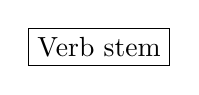
\begin{tikzpicture}[remember picture, baseline=(stem.base)] \node [draw] (stem) {Verb stem};\end{tikzpicture} & -\oneP\slash{\twoP} subject\# & direct object & =adpositional & =directional & =Perfect\\
derivational prefix- &  &  & {}-indirect object  & pronominal & & & \\
 & & & pronominal\# & \begin{tikzpicture}[remember picture] 
 \draw [overlay,thick, -{Stealth}] (Fig2wordL.north) -- (Fig2L.north east);
 \draw [overlay,thick, -{Stealth}] (Fig2wordR.north) -- (Fig2C.north west);
 \draw [overlay,thick, -{Stealth}] (Fig2extR.north) -- (Fig2R.north east);
  \end{tikzpicture}\\
 \end{tabular}}
\caption{Two phonological word verb complex\label{fig:7.2}\label{fig:12}}
\end{figure}

The word break is initiated by both the direct and indirect object pronominals such that when either is present, there will be a word break. The word break after the \oldstylenums{3}\textsc{s} indirect object pronominal enclitic is indicated by word-final changes in /n/; in slow speech the \oldstylenums{3}\textsc{s} indirect object pronominal enclitic /=\textit{an }/ is pronounced [aŋ] (showing word-final changes) even when there are other clitics following the verb word (\ref{ex:7:3}, see \sectref{sec:7.3.1.1}).  The word break before the \oldstylenums{3}\textsc{s} \DO pronominal is indicated by the fact that the \oldstylenums{3}\textsc{s} \DO pronominal does not neutralise the prosody on the verb stem, and does not cause the  /-j/ suffix to drop (\ref{ex:7:4} and \ref{ex:7:5}, see \sectref{sec:7.3.2}).\footnote{The first line in each example is the orthographic form. The second is the phonetic form (slow speech) with morpheme breaks.} 


\ea\label{ex:7:3}
Ambaɗan  aka  alay.\\
verb word   \hspace{50pt}  ‘extension word’\\
\gll [à-mbaɗ  =aŋ] \hspace{5pt} [=aka  =alaj]\\
\oldstylenums{3}\textsc{s}+{\PFV}-change =\oldstylenums{3}\textsc{s}.{\IO} \hspace{5pt}  =on   =away\\
\glt ‘He/she replied.’ (lit. he changed on away)
\z

\ea\label{ex:7:4}
Aslay na.\\
\gll {}[à-ɬ{}-aj] \hspace{35pt}   [na]\\
\oldstylenums{3}\textsc{s}+{\PFV}-slay-{\CL} {} \oldstylenums{3}\textsc{s}.{\DO}\\
\glt ‘He killed it.’
\z

\ea\label{ex:7:5}
Ege   na.\\
\gll {}[\`ɛ-g-ɛ]  \hspace{45pt}  [na]\\
\oldstylenums{3}\textsc{s}+{\PFV}-do -{\CL}{} \oldstylenums{3}\textsc{s}.{\DO}\\
\glt ‘He did it.’
\z

 \REF{ex:7:6} shows a direct object pronominal with no indirect object pronominal enclitic and the extensions cliticise to the direct object pronominal.  \REF{ex:7:7} shows both direct and indirect object pronominals; again the extensions cliticise to the direct object pronominal.  \REF{ex:7:3} and \REF{ex:7:8} show an indirect object pronominal enclitic with no direct object pronominal. When there is no direct object pronominal, the extensions form a separate phonological word in and of themselves. 

\ea\label{ex:7:6}
Abək  ta  aya  va  məlama  ahan  ahay  jəyga.\\
 verb word \hspace{9pt} ‘extension word’\\
\gll {}[a-bək] \hspace{15pt}  [ta=aja=va]  \hspace{10pt}  məlama  =ahaŋ    =ahaj  dzijga\\
\oldstylenums{3}\textsc{s}-invite \hspace{15pt}  \oldstylenums{3}\textsc{p}.{\DO}={\PLU}={\PRF} {}  brothers  =\oldstylenums{3}\textsc{p}.{\POSS}  =Pl  all\\
\glt ‘He had already invited all of his brothers.’  
\z

\ea\label{ex:7:7}
Akaɗaw  na  va. \\
verb word  \hspace{36pt}        ‘extension word’\\
\gll {}[à-kaɗ  =aw]    [na  =va]\\
\oldstylenums{3}\textsc{s}+{\PFV}-club ={\oneS}.{\IO}    \oldstylenums{3}\textsc{s}.{\DO}  ={\PRF}\\
\glt ‘He/she has killed it for me.’ 
\z

\ea\label{ex:7:8}
Hor  agaw  aka  ala.\\
\hspace{30pt} verb word \hspace{28pt} ‘extension word’\\
\gll hʷɔr    [à-g=aw]     [=aka   =ala]\\
woman  \oldstylenums{3}\textsc{s}+{\PFV}-do=\oldstylenums{3}\textsc{s}.{\IO}   =on   =to\\
\glt ‘The woman liked me [as I liked her].’ (lit. she did to me on toward)  
\z

The third type of verb complex consists of three phonological words (a verb word, an ‘indirect object word,’ and an ‘extension word’). This type occurs when the verb complex has both a subject suffix and an indirect object pronominal enclitic. Phonological rules will not allow two morphemes suffixed or cliticised to the verb; nor can the indirect object pronominal enclitic commence another word. So, the morpheme \textit{an} is inserted and the indirect object pronominal clitic attaches to the inserted morpheme. The overall structure is then as shown in \figref{fig:7.3}.

\begin{figure}
\resizebox{\textwidth}{!}{%
\begin{tabular}{llll|l|llll}
\tikzmark{Fig3L}   & \multicolumn{2}{c}{\tikzmark{Fig3wordL} Verb word \tikzmark{Fig3wordR}} \tikz[remember picture] \draw[overlay, thick, {Stealth}-] (Fig3L.north west) -- (Fig3wordL.north);  & \multicolumn{1}{r|}{\tikzmark{Fig3VWR}\tikz[remember picture] \draw[overlay, thick, {Stealth}-] (Fig3VWR.north east) -- (Fig3wordR.north);}   & Indirect object word & \multicolumn{3}{l}{Extension word \tikzmark{Fig3Ext}} & \multicolumn{1}{r}{\tikzmark{Fig3R}} \tikz[remember picture] \draw[overlay, thick, {Stealth}-] (Fig3R.north east) -- (Fig3Ext.north);\\
%                    & \multicolumn{2}{c}{}          &                      &                      & \\
                   \multicolumn{4}{r|}{} & & \\
subject & Irrealis- & \tikz[baseline=(verbstem.base)] \node [draw] (verbstem) {\strut Verb stem}; & -\oneP\slash{\twoP} & an=indirect  & direct object & =adpositional & =directional & =Perfect\\
+\textsc{aspect}-  &  &	  & subject\#    & object pronominal\#  & pronominal    &          &         &    \\
\end{tabular}}
\caption{Three phonological word verb complex\label{fig:7.3}}
\end{figure}

In \REF{ex:7:9} and \REF{ex:7:10}, the verb \textit{kəslom }has the {\twoP} imperative suffix attached (\textit{-om}). The indirect object pronominal enclitic and the inserted morpheme \textit{an}. Other extensions must make a third phonological word since there is a word break following the indirect object pronominal enclitic. 


\ea\label{ex:7:9}
Kəslom  anan  na  aka  awak.\\
verb word   \hspace{10pt}        ‘indirect object word’   \hspace{10pt}    ‘extension word’\\
\gll  [kʊ-ɬ-ɔm] \hspace{15pt}   [an=aŋ] \hspace{60pt}   [na  =aka] \hspace{30pt}   awak\\
2-slay-{\twoP} \hspace{15pt} {\DAT}=\oldstylenums{3}\textsc{s}.{\IO} \hspace{60pt}   \oldstylenums{3}\textsc{s}.{\DO}  =on \hspace{30pt}   goat\\
\glt ‘You (p) kill another goat for him.’ (lit. you slay a goat for him on top of [another time a goat was slain]
\z

\ea\label{ex:7:10}
 Kəslom  anan  aka  awak.\\
verb word    \hspace{10pt}             ‘indirect object word’ \hspace{10pt} ‘extension word’\\
\gll {}[kʊ-ɬ-ɔm] \hspace{15pt} [an=aŋ] \hspace{60pt} [=aka] \hspace{50pt}   awak\\
2-kill-{\twoP} \hspace{15pt} {\DAT}=\oldstylenums{3}\textsc{s}.{\IO} \hspace{60pt} =on \hspace{50pt}   goat\\
\glt ‘You kill another goat for him.’
\z
The three types of verb complexes seen in Moloko are shown in \figref{tab:53}.

\begin{figure}
\resizebox{\textwidth}{!}{\begin{tabular}{llllllllll}
1 & \tikzmark{Fig4-1L} & \multicolumn{4}{c}{\tikzmark{Fig4-1VWL} Verb word \tikzmark{Fig4-1VWR}} & \multicolumn{1}{r}{\tikzmark{Fig4-1R}}
    \begin{tikzpicture}[remember picture] 
	\draw[overlay, thick, {Stealth}-] (Fig4-1L.north west) -- (Fig4-1VWL.north); 
	\draw[overlay, thick, -{Stealth}] (Fig4-1VWR.north) -- (Fig4-1R.north east);
    \end{tikzpicture}\\
    \\
  &   subject+\textsc{aspect}- & Irrealis- & 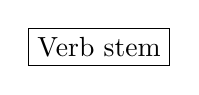
\begin{tikzpicture}[remember picture, baseline=(stem.base)] \node [draw] (stem) {Verb stem};\end{tikzpicture} & =adpositional & =directional & =Perfect\\
  \\
2 & \tikzmark{Fig4-2L} & & \tikzmark{Fig4-2wordL} Verb word \tikzmark{Fig4-2wordR} & \multicolumn{1}{r|}{\tikzmark{Fig4-2C}} & \multicolumn{2}{l}{Extension word \tikzmark{Fig4-2extR}} & & \multicolumn{1}{r}{\tikzmark{Fig4-2R}}\\
  & \multicolumn{4}{r|}{}\\
  & subject+\textsc{aspect}- & Irrealis- & 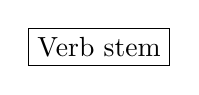
\begin{tikzpicture}[remember picture, baseline=(stem.base)] \node [draw] (stem) {Verb stem};\end{tikzpicture} & \multicolumn{1}{l|}{-\oneP\slash{\twoP} subject\#} & direct object & =adpositional & =directional & =Perfect\\
  & derivational prefix- &  &  & \multicolumn{1}{l|}{-indirect object\#}  & pronominal & & & \\
    \begin{tikzpicture}[remember picture]
    \draw[overlay, thick, -{Stealth}] (Fig4-2wordL.north) -- (Fig4-2L.north west);
    \draw[overlay, thick, -{Stealth}] (Fig4-2wordR.north) -- (Fig4-2C.north east);
    \draw[overlay, thick, -{Stealth}] (Fig4-2extR.north) -- (Fig4-2R.north east);
    \end{tikzpicture}\\
3 &\tikzmark{Fig4-3L}   & \multicolumn{2}{c}{\tikzmark{Fig4-3wordL} Verb word \tikzmark{Fig4-3wordR}} \tikz[remember picture] \draw[overlay, thick, {Stealth}-] (Fig4-3L.north west) -- (Fig4-3wordL.north);  & \multicolumn{1}{r|}   {\tikzmark{Fig4-3VWR}\tikz[remember picture] \draw[overlay, thick, {Stealth}-] (Fig4-3VWR.north east) -- (Fig4-3wordR.north);}   & \multicolumn{1}{l|}{Indirect object word} & \multicolumn{3}{l}{Extension word \tikzmark{Fig4-3Ext}} & \multicolumn{1}{r}{\tikzmark{Fig4-3R}} \tikz[remember picture] \draw[overlay, thick, {Stealth}-] (Fig4-3R.north east) -- (Fig4-3Ext.north);\\
%                    & \multicolumn{2}{c}{}          &                      &                      & \\
  & \multicolumn{4}{r|}{} & \multicolumn{1}{r|}{}& \\
  & subject +\textsc{aspect}- & Irrealis- & \tikz[baseline=(verbstem.base)] \node [draw] (verbstem) {\strut Verb stem}; & \multicolumn{1}{l|}{-\oneP\slash{\twoP} subject\#} & \multicolumn{1}{l|}{an=indirect} & direct object & =adpositional & =directional & =Perfect\\
  &   &	   &	       &     \multicolumn{1}{r|}{}       & \multicolumn{1}{l|}{object pronominal\#}  & pronominal    &               &              &      \\
\end{tabular}}
\caption{Three types of verb complexes\label{tab:53}}
\end{figure}

\section{Imperative}\label{sec:7.2}
\hypertarget{RefHeading1212121525720847}{}
The {\twoS} imperative form is the basic citation form of the verb as the {\twoS} form gives the clearest presentation of the verb stem. The imperative occurs in {\twoS}, \oldstylenums{1}\textsc{Pin} and {\twoP} forms. The {\twoS} form is simply the verb stem. The plural\is{Plurality!Verb plurals|(} forms carry suffixes which correspond to their respective subject pronominal suffixes in indicative verb stems (see \sectref{sec:7.3.1}). The singular and plural imperative forms are shown in \tabref{tab:54}. (from \citealt{FriesenMamalis2008}). 

\begin{table}
\begin{tabular}{lll}
\lsptoprule
{\twoS} form & {\oneP inclusive form} & {{\twoP} form}\\\midrule
\textit{faɗ} & \textit{fəɗ{}-ok} & \textit{fəɗ{}-om}\\
‘Put! ({\twoS})’ & ‘Let’s put! (\oldstylenums{1}\textsc{Pin})’ & ‘Put! ({\twoP})’\\\midrule
\textit{zom}~ & \textit{zəm-ok} & \textit{zəm-om}\\
‘Eat! ({\twoS})’ & ‘Let’s eat! (\oldstylenums{1}\textsc{Pin})’ & ‘Eat! ({\twoP})’\\\midrule
\textit{s{}-e} & \textit{s-ok} & \textit{s-om}\\
‘Drink! ({\twoS})’ & ‘Let’s drink! (\oldstylenums{1}\textsc{Pin})’ & ‘Drink! ({\twoP})’\\\midrule
\textit{fat-ay} & \textit{fot-ok} & \textit{fot-om}\\
‘Descend! ({\twoS})’ & ‘Let’s descend! (\oldstylenums{1}\textsc{Pin})’ & ‘Descend! ({\twoP})’\\
\lspbottomrule
\end{tabular}
\caption{Singular and plural imperative forms\label{tab:54}}
\end{table}

\section{Verb complex pronominals}\label{sec:7.3}
\hypertarget{RefHeading1212141525720847}{}
\citet{FriesenMamalis2008} showed that the verb complex can carry pronominals that indicate the subject, direct object, and indirect object. These markers in the verb complex are all bound forms. They are called pronominals and not just agreement markers because all of them can be the only indication of their referent in the clause. Because the pronominals are present, there is no need for a noun phrase or free pronoun in the clause. Participants are tracked\is{Cohesion!Participant tracking} in discourse solely by pronominals, and free pronouns and noun phrases only occur in discourse to introduce a participant or to switch the referent. 


\tabref{tab:55} lists all the pronominals.  Subject is indicated by a verbal prefix for singular subjects and third person plural.  Plural subjects for first and second person are indicated by a combination of a prefix and a suffix. These subject pronominals (discussed in \sectref{sec:7.3.1}) are given in their underlying form because the surface vowel and tone on the prefix is determined by mood and aspect, respectively. Also, the underlying form is given to show the prosody, because the labialisation prosody in the plural subject suffixes will spread over the entire verb stem. The direct object pronominal (\sectref{sec:7.3.2}) only occurs for third person singular and plural. The indirect object pronominal (\sectref{sec:7.3.1.1}) cliticises to the right edge of the verb stem and the direct object pronominal follows it. In \tabref{tab:55}, the independent pronouns are also given for comparison since there are similarities between the free pronoun and its corresponding pronominal.

\begin{table}
\resizebox{\textwidth}{!}{\begin{tabular}{lllll}
\lsptoprule
{Person} & {Pronominal} & {Indirect object} & {Third person} & {Independent}\\
& {subject affixes} & {pronominal } & {direct object} & {pronouns}\\
& & {enclitics} & {pronominals} & \\\midrule
{{\oneS}} & \textit{n-} & =\textit{aw} &  & \textit{ne}\\
{{\twoS}} & \textit{k-} & =\textit{ok} &  & \textit{nok}\\
{\oldstylenums{3}\textsc{s}} & \textit{a-} / \textit{ma-}\footnote{The third person Hortative subject pronominal, see \tabref{tab:65} in \sectref{sec:7.4.3}.} & \textit{=an} & \textit{na} & \textit{ndahan}\\
{\oneP inclusive\footnote{i.e. speaker (+others)  + hearer} } & \textit{m-}…-\textit{ok} & \textit{=aloko} &  & \textit{loko}\\
{\oneP exclusive\footnote{i.e. speaker + others}} & \textit{n-}…-\textit{om} & \textit{=aləme} &  & \textit{ləme}\\
{{\twoP}} & \textit{k-}…-\textit{om} & \textit{=aləkwəye} &  & \textit{ləkwəye}\\
{\oldstylenums{3}\textsc{p}} & \textit{t-} & \textit{=ata} & \textit{ta} & \textit{təta}\\
\lspbottomrule
\end{tabular}}
\caption{Pronominals}\label{tab:55}
\end{table}

\subsection{Subject pronominal affixes}\label{sec:7.3.1}
\hypertarget{RefHeading1212161525720847}{}
The subject is always marked on the finite form of the verb, regardless of whether there is a free subject phrase in the clause.\footnote{The presence of both subject pronominal and corresponding noun phrase occurs for pragmatic reasons.}  In fact, the subject pronominal marker in the verb can be the only indication of subject in the entire clause.\footnote{In a non-finite verb form, the subject pronominal is absent and the subject of the clause is either understood from the context or indicated by a free pronoun or noun phrase in the clause (Sections \ref{sec:7.6.2}, \ref{sec:7.7}, and \ref{sec:8.2.3}).} As noted in \tabref{tab:56} and \tabref{tab:57} (adapted from \citealt{FriesenMamalis2008}), subject is marked by a prefix or combination of prefix and suffix. In the examples below, the pronominal affixes are bolded. The prefix carries aspectual tone (see \sectref{sec:7.4}), and the vowel quality is influenced by the prosody on the verb stem (see \sectref{sec:6.6}), the presence of the /a-/ prefix (see \sectref{sec:6.5}), and the mood of the verb (see \sectref{sec:7.4.3}). The \oneP and {\twoP} suffixes are labialised. This prosody will spread over the entire verb stem. 

\begin{table}
\begin{tabular}{lll}
\lsptoprule
{Person} & {Singular} & {Plural}\\\midrule
{1} & \textit{\textbf{nə-}mənjar awak} & \textbf{\textit{mə-}}\textit{mənjor}\textbf{\textit{{}-ok}} \textit{awak}\\
& ‘I saw a goat’ & ‘we (inclusive) saw a goat’\\
&  & \textbf{\textit{nə-}}\textit{mənjor}\textbf{\textit{{}-om}} \textit{awak}\\
& & ‘we (exclusive) saw a goat’\\\midrule
{2} & \textbf{\textit{kə-}}\textit{mənjar awak} & \textbf{\textit{kə-}}\textit{mənjor-}\textbf{\textit{om}} \textit{awak}\\
& ‘you saw a goat’  & ‘you (plural) saw a goat’\\\midrule
{3} & \textbf{\textit{a-}}\textit{mənjar awak} & \textbf{\textit{tə-}}\textit{mənjar awak}\\    
& ‘he/she saw a goat’  & ‘they saw a goat’\\
\lspbottomrule
\end{tabular}
\caption{Conjugations with subject pronominal affixes for the verb /m nzar/ ‘see’}\label{tab:56}
\end{table}

\begin{table}
\begin{tabular}{lll}
\lsptoprule
{Person} & {Singular} & {Plural}\\\midrule
{1} & \textbf{\textit{nə-}}\textit{həm-ay} & \textbf{\textit{mə{}-}}\textit{həm}\textbf{\textit{{}-ok}}  \\
& ‘I ran’ & ‘we (inclusive) ran’\\
&  & \textbf{\textit{nə{}-}}\textit{həm}\textbf{\textit{{}-om}} \\  
& & ‘we (exclusive) ran’\\\midrule
{2} & \textbf{\textit{kə-}}\textit{həm-ay}  & \textbf{\textit{kə{}-}}\textit{həm}\textbf{\textit{{}-om}}\\
& ‘you ran’ & ‘you (plural) ran’\\\midrule
{3} & \textbf{\textit{a-}}\textit{həm-ay} & \textbf{\textit{tə-}}\textit{həm-ay}\\
& ‘he/she ran’ & ‘they ran’\\
\lspbottomrule
\end{tabular}
\caption {\label{tab:57} Conjugations with subject pronominal affixes for the verb /h m-aj/ ‘run’}
\end{table}

\largerpage \citet{Bow1997c} found that a prosody on the verb stem will spread leftwards from the verb stem over the singular subject prefixes. The fact that palatalisation and labialisation spread over the subject prefixes indicates that the subject markers are fully bound to the verb stem and are not separate words. \REF{ex:7:11} presents the palatalised verb / g\textsuperscript{ e}\textit{ }/ ‘do,’ and \REF{ex:7:12} presents the labialised verb / l\textsuperscript{o}/ ‘go.’  

\ea\label{ex:7:11}
Nege.\\
\gll {}[nɛ\textbf{{}-}g-ɛ]\\
{\oneS}-do-{\CL}\\
\glt ‘I did.’
\z

\ea\label{ex:7:12}
Olo.\\
\gll {}[ɔ\textbf{{}-}lɔ]\\
\oldstylenums{3}\textsc{s}-go\\
\glt ‘he/she went.’
\z

\citet{Bow1997c} also discovered that labialisation on the {\oneP} and {\twoP} subject suffixes will spread leftwards from the suffix onto the entire verb word. This fact indicates that these morphemes are fully bound to the verb stem and are not separate words.  The verb / ts k -j\textsuperscript{ e }/ ‘stand’, shown in example \REF{ex:7:13} in its {\oneS} form, loses its palatalisation and becomes labialised when the (labialised) plural\is{Plurality!Verb plurals|)} suffixes are added \REF{ex:7:14}:

\ea\label{ex:7:13}
Necəke.\\
\gll nɛ\textbf{{}-}tʃɪk-ɛ\\
{\oneS}-stand-{\CL}    \\
\glt ‘I stand.’
\z

\ea\label{ex:7:14}
Nəcəkom.    \\
\gll nʊ\textbf{{}-}tsʊkʷ{}-ɔm\\
\oldstylenums{1}-stand-\oldstylenums{1}\textsc{Pex}\\
\glt ‘We (exclusive) stand.’
\z

\citet{Bow1997c} also determined that the subject pronominal prefixes in Moloko appear to be toneless. The aspect of the verbal construction will allocate tone to the pronoun.   In the Imperfective aspect\is{Tense, mood, and aspect!Imperfective aspect}, the pronoun always takes high tone (see \sectref{sec:7.4.2}).  In the Perfective aspect\is{Tense, mood, and aspect!Perfective aspect}, the pronoun copies the first tone of the root if it is low or mid.  If the first tone of the root is high, the pronoun takes on mid tone.

\subsection{Indirect object pronominal enclitic}\label{sec:7.3.1.1}

An indirect object pronominal enclitic can attach to the verb word to express the indirect object, which is a core argument of the verb. The indirect object in Moloko is the participant that represents the place where the direct object is directed to – the recipient or beneficiary of the action.\footnote{Employing the Agent-Theme-Location analysis developed by \citet{DeLancey1991}, the indirect object in Moloko expresses the semantic \LOC (see \chapref{chap:9}). The direct object pronominal expresses the semantic Theme -- the participant that changes position or state (see \sectref{sec:7.3.2}).} In \REF{ex:7:15}, the verb /dz -j/ ‘help’ takes the indirect object. The indirect object represents the participant who receives the help. 


\ea\label{ex:7:15}
Ajənaw.\\
\gll a-dzən =aw\\
\oldstylenums{3}\textsc{s}-help  ={\oneS}.{\IO}\\
\glt ‘He/she helped me.’
\z

The indirect object pronominal enclitic allows the core indirect object argument to be expressed in a prepositional phrase \textit{ana Mana} ‘to Mana’ \REF{ex:7:16}. 

\ea\label{ex:7:16}
Ajənan ana Mana.\\
\gll a-dzən  =aŋ  ana  Mana\\
\oldstylenums{3}\textsc{s}-help  =\oldstylenums{3}\textsc{s}.{\IO}  {\DAT} Mana\\
\glt ‘He/she helped Mana.’
\z

The indirect object pronominal enclitic can also stand in the place of the prepositional phrase \REF{ex:7:17}.

\ea\label{ex:7:17}
Ajən\textbf{an}.\\
\gll a-dzən  \textbf{=aŋ}\\
\oldstylenums{3}\textsc{s}-help  =\oldstylenums{3}\textsc{s}.{\IO}\\
\glt ‘He/she helped him.’
\z

\tabref{tab:7.58} (adapted from \citealt{FriesenMamalis2008}) shows the verb /v l/ ‘give’ conjugated for the indirect object argument. The indirect object expresses the recipient.

\begin{table}
\begin{tabular}{lll}
\lsptoprule
{Person} & {Singular} & {Plural}\\\midrule
{1} & \textit{a-vəl\textbf{=aw}}  & \textit{a-vəl}\textbf{\textit{=aloko}}\\
& ‘he/she gave to me’ & ‘he/she gave to us (inclusive)’\\
&  & \textit{a-vəl}\textbf{\textit{=aləme}}\\
& & ‘he/she gave to us (exclusive)’\\\midrule
{2} & \textit{a-vəl}\textbf{\textit{=ok}} & \textit{a-vəl}\textbf{\textit{=aləkwəye}}\\
& ‘he/she gave to you’ & ‘he/she gave to you (plural)’\\\midrule
{3} & \textit{a-vəl}\textbf{\textit{=an}} & \textit{a-vəl}\textbf{\textit{=ata}}\\
& ‘he/she gave to him/her’ & ‘he/she gave to them’\\
\lspbottomrule
\end{tabular}
\caption{Verb /v l/ ‘give’ conjugated for indirect object pronominal enclitic\label{tab:7.58}}
\end{table}

The indirect object pronominal enclitics are phonologically bound to the verb stem  and do not comprise separate words.  When an indirect object pronominal cliticises to the verb stem, there are no word final alternations in the verb stem. Compare the following pairs of examples showing verb stems with and without indirect object pronominal enclitics. \REF{ex:7:18} and \REF{ex:7:19} show that when the indirect object pronominal enclitic is attached \REF{ex:7:19}, we do not see the word final alternation of /h/ → [x] / \_\#.\footnote{See \sectref{sec:2.6.1}. Likewise, we do not see the word-final process of n → [ŋ] /  \_\# between the verb stem and the indirect object pronominal.} 

\ea\label{ex:7:18}
Aɓah  zana.\\
\gll a-ɓax  zana\\
\oldstylenums{3}\textsc{s}-sew    clothing\\
\glt ‘He/she sews clothing.’
\z

\ea\label{ex:7:19}
Aɓahaw  zana.  \\
\gll a-ɓah=aw    zana  \\
\oldstylenums{3}\textsc{s}{}-sew={\oneS}.{\IO}   clothing    \\
\glt ‘He/she sews clothing for me.’
\z

Similarly, the example pairs \REF{ex:7:20} and \REF{ex:7:21} illustrate that the /-j/ suffix is dropped when the indirect object pronominal is present \REF{ex:7:21}, indicating that the pronominal is phonologically bound to the stem (see \sectref{sec:6.3}). 

\ea\label{ex:7:20}
Ajay.\\
\gll a-dz-aj\\
\oldstylenums{3}\textsc{s}-speak{}-{\CL}\\
\glt ‘He/she speaks.’
\z

\ea\label{ex:7:21}
Ajan.\\
\gll a-dz=aŋ\\
\oldstylenums{3}\textsc{s}-speak=\oldstylenums{3}\textsc{s}.{\IO}\\
\glt ‘He/she speaks to him/her.’
\z

The indirect object pronominal enclitic is not phonologically a true suffix, because the prosody of the indirect object pronominal enclitic does not affect the prosody on the verb stem. Compare \REF{ex:7:22} and \REF{ex:7:23} which illustrate the verb stem /s/ conjugated with second person singular and plural indirect objects. If the prosody of the indirect object pronominal enclitic affected the verb stem, one would expect that the /s/ in example \REF{ex:7:23} would be affected by the palatalisation prosody of the plural indirect object pronominal enclitic and be expressed as [ʃ]. 

\ea\label{ex:7:22}
Asok  aka  ɗaf.\\
\gll a-s=ɔk    =aka  ɗaf\\
\oldstylenums{3}\textsc{s}-please={\twoS}.{\IO}  =on  {millet loaf}\\
\glt ‘You  want to have more millet loaves.’ (lit. millet loaf is pleasing to you)  
\z

\ea\label{ex:7:23}
Asaləkwəye  aka  ɗaf.\\
\gll a-s=alʊkʷøjɛ  =aka ɗaf\\
\oldstylenums{3}\textsc{s}-please={\twoP}.{\IO}  =on  {millet loaf}\\
\glt ‘You want to have more millet loaves.’ (lit. millet loaf is pleasing to you)  
\z

The fact that the indirect object pronominal can attach to verb stems as well as other particles confirms that it is in fact a clitic pronoun. Normally, the indirect object pronominal enclitic attaches directly to the verb stem \REF{ex:7:24}.  However, if the plural subject pronominal suffix is required on the verb \REF{ex:7:25}, the indirect object pronominal can no longer attach to the verb, because the verb stem can take only one suffix (see \sectref{sec:7.1}). Instead, the indirect object pronominal cliticises to the particle \textit{an}\textit{.} This particle may be related to \textit{ana}, the dative preposition ‘to.’

\ea\label{ex:7:24}
Kasl\textbf{an}  awak.\\
\gll ka-ɬ\textbf{=aŋ}      awak\\
{\twoS}-slay=\oldstylenums{3}\textsc{s}.{\IO}    goat\\
\glt ‘You slay the goat for him.’ 
\z

\ea\label{ex:7:25}
Kəslom  \textbf{anan}  awak.\\
\gll kə-ɬ{}-ɔm  \textbf{an=aŋ}    awak\\
\oldstylenums{2}-slay-{\twoP}  to=\oldstylenums{3}\textsc{s}.{\IO}  goat\\
\glt ‘You (plural) slay the goat for him.’  
\z

There is a word break after the indirect object pronominal enclitic (the phonological words are indicated by square brackets in the examples immediately below).  The word break is indicated by the fact that the \oldstylenums{3}\textsc{s} indirect object pronominal enclitic /=\textit{an}/ in slow speech is pronounced [aŋ] even when there are other clitics following the verb word (see \ref{ex:7:26} and \ref{ex:7:27}). The word-final [ŋ] will delete in fast speech (see \sectref{sec:2.5.2}). These clitics (e.g., the adpositional clitics in these examples, see \sectref{sec:7.5.1}) would otherwise attach to the verb (compare with example \ref{ex:7:28}):

\ea\label{ex:7:26}
As\textbf{an}  \textbf{aka}  ɗaf.\\
\gll {}[a-s\textbf{=aŋ}] [\textbf{=aka}]    ɗaf\\
\oldstylenums{3}\textsc{s}-please=\oldstylenums{3}\textsc{s}.{\IO}  =on    {millet loaf}\\
\glt ‘He/she wants to have more millet loaves.’ (lit. millet loaf is pleasing to him)  
\z

\ea\label{ex:7:27}
Ad\textbf{an}  \textbf{aka}  ɗaf.\\
\gll {}[a-d\textbf{=aŋ}] [\textbf{=aka}]    ɗaf\\
\oldstylenums{3}\textsc{s}-prepare=\oldstylenums{3}\textsc{s}.{\IO}  =on    {millet loaf}\\
\glt ‘She made more loaves of millet for him.’
\z

\ea\label{ex:7:28}
Ad\textbf{aka}  ɗaf.\\
\gll {}[a-d \textbf{=aka}]        ɗaf\\
\oldstylenums{3}\textsc{s}-prepare =on      {millet loaf}\\
\glt ‘She made more loaves of millet.’  
\z

\subsection{Third person direct object pronominal}\label{sec:7.3.2}
\hypertarget{RefHeading1212181525720847}{}
\tabref{tab:55} (from \citealt{FriesenMamalis2008}) shows the direct object (\DO) pronominals. The third person \DO pronominals replace or double a full noun phrase in a discourse -- the \textit{na} (\oldstylenums{3}\textsc{s}.{\DO}) or \textit{ta} (\oldstylenums{3}\textsc{p}.{\DO}) refer back to something in the immediately preceding context. \REF{ex:7:29} and \REF{ex:7:30} show two clauses that might occur in a discourse. In \REF{ex:7:30} the \textit{na} refers back to \textit{sla} ‘cow’ in \REF{ex:7:29}.

\ea\label{ex:7:29}
Kaslay  sla.   \\   
\gll kà-ɬ{}-aj    ɬa  \\    
{\twoS}+{\PFV}-slay{}-{\CL}  cow  \\       
\glt ‘You slew the cow.’            
\z

\ea\label{ex:7:30}
Kaslay  \textbf{na}\textbf{.}\\
\gll kà-ɬ{}-aj     \textbf{na}\\
{\twoS}+{\PFV}-slay{}-{\CL}    \oldstylenums{3}\textsc{s}.{\DO}  \\
\glt ‘You slew it.’
\z

A third person \DO pronominal can be the only expression of direct object in a clause if its identity is known in the discourse (\ref{ex:7:30}, \ref{ex:7:32}, and \ref{ex:7:36}). The only time that a clause will contain both a third person \DO pronominal and a noun phrase that co-refer to the direct object in the clause is when a special focus on the direct object is required (‘all his brothers’ in \ref{ex:7:31}, ‘that fruit-bearing tree’ in \ref{ex:7:38}). 


\ea\label{ex:7:31}\corpussource{Race Story\footnote{\citealt{Friesen2003}.}}\\
Moktonok  na,  abək  \textbf{ta}  aya  va  məlama  ahan  ahay  jəyga.\\
\gll mɔkʷtɔnɔkʷ na  a-bək       \textbf{ta}=aja=va  məlama  =ahaŋ    =ahaj  dzijga\\
toad    {\PSP}  \oldstylenums{3}\textsc{s}-invite  \oldstylenums{3}\textsc{p}={\PLU}={\PRF}  brothers  =\oldstylenums{3}\textsc{p}.{\POSS}  =Pl  all\\
\glt ‘The toad, he had already invited all of his brothers.’  
\z

We know that the third person \DO pronominals are phonologically separate words (not clitics like the other verbal extensions) because the /-j/ suffix does not drop when the \DO pronominal is added to a clause \REF{ex:7:32}.  Normally the /-j/ suffix drops off when extensions or suffixes are added to the clause (\ref{ex:7:33}, see also \sectref{sec:6.3}). 

\ea\label{ex:7:32}
Apaɗay  \textbf{na}.   \\   
\gll a-paɗ-aj     \textbf{na} \\     
\oldstylenums{3}\textsc{s}-crunch{}-{\CL}   \oldstylenums{3}\textsc{s}.{\DO}\\
\glt ‘He/she crunches it.’ 
\z

\ea\label{ex:7:33}
Apaɗaka.\\
\gll a-paɗ  =aka\\
\oldstylenums{3}\textsc{s}-crunch  =on\\
\glt ‘He/she crunches on.’ 
\z

Another indication that the \DO pronominal is phonologically a separate word is that the neutral prosody on the \DO pronominal does not affect the prosody of the verb word. Compare \REF{ex:7:34} and \REF{ex:7:35}. In both examples the verb complex is palatalised in spite of the addition of the \DO pronominal. This situation is in contrast to what happens with the Perfect enclitic (see \sectref{sec:7.5.3}). 

\ea\label{ex:7:34}
Nese.\\
\gll nɛ-ʃ{}-ɛ\\
{\oneS}-drink{}-{\CL}\\
\glt ‘I drink.’
\z

\ea\label{ex:7:35}
Nese  na.\\
\gll nɛ-ʃ{}-ɛ  na\\
{\oneS}-drink{}-{\CL}  \oldstylenums{3}\textsc{s}.{\DO}\\
\glt ‘I drink it.’ 
\z

A third indication is that word final changes (like word-final /n/ being realised as [ŋ] (see \sectref{sec:2.6.1} and example \ref{ex:7:36}) are preserved when followed by \textit{na} or \textit{ta}.

\ea\label{ex:7:36}
Nəvəlan  \textbf{na}. \\
\gll nə-vəl=aŋ     \textbf{na} \\
{\oneS}-give=\oldstylenums{3}\textsc{s}.{\IO}   \oldstylenums{3}\textsc{s}.{\DO}\\
\glt ‘I gave it to him.’
\z

The normal slot for the \DO pronominal is within the verb complex between the verb stem and the directional extension. In each example below, the verb complex is delineated by square brackets and the third person \DO pronominal is bolded.

\ea\label{ex:7:37}
Baba  ango  avəlan  \textbf{na}  alay  ana  məze.\\
\gll baba  =aŋgʷɔ  [a-vəl=aŋ  \textbf{na} =alaj]  ana  mɪʒɛ\\
father  ={\twoS}.{\POSS}  \oldstylenums{3}\textsc{s}-give=\oldstylenums{3}\textsc{s}.{\IO}  \oldstylenums{3}\textsc{s}.{\DO} =away    {\DAT} person\\
\glt ‘Your father gave it to that person.’  
\z

Any further verbal extensions will cliticise to a third person \DO pronominal. In example \REF{ex:7:38}, the directional extension \textit{=ala} ‘toward’ cliticises to \textit{na} and vowels will elide resulting in the pronunciation [nala]. See also example \REF{ex:7:31}, where the pluractional and perfect extensions \textit{=}\textit{aya} and \textit{=}\textit{va} cliticise to the \DO pronominal \textit{ta} to result in the pronunciation [tajava].  


\ea\label{ex:7:38}\corpussource{Cicada, S. 12}\\
Tolo  [təmənjar  \textbf{na}  ala]  mama  agwazla  nəndəye.\\
\gll tɔ{}-lɔ    [tə-mənzar  \textbf{na} =ala] mama  agʷaɮa   nɪndijɛ\\
\oldstylenums{3}\textsc{p}-go  \oldstylenums{3}\textsc{p}-see   \oldstylenums{3}\textsc{s}.{\DO}   =to  mother  {spp. of tree}  {\DEM}\\
\glt ‘They went and saw that fruit-bearing tree.’
\z

\largerpage
The first and second person direct objects are expressed by free pronouns (see \sectref{sec:3.1.1.1}) or noun phrases. The free pronouns are distributionally and phonologically distinct from the third person direct object pronominals. The free pronouns occur after the verb complex. Note that they occur after the directional extensions in \REF{ex:7:39} and \REF{ex:7:40}. In each example, the verb complex is delineated by square brackets and the first or second person independent pronoun is bolded.

\ea\label{ex:7:39}
[Kazalay]  \textbf{ne}  a  kosoko  ava  ɗaw?\\
\gll {}[ka-z  =alaj]    \textbf{nɛ}  a  kɔsɔkʷɔ  ava  ɗaw\\
{\twoS}-take  =away    {\oneS}  at  market  in  {\QUEST}\\
\glt ‘Will you take me to the market?’
\z

\ea\label{ex:7:40}
Baba  ango  [avəlata]  \textbf{nok}  va  a  ahar  ata  ava\\
\gll baba  =aŋgʷɔ    [à-vəl=ata]  \textbf{nɔkʷ}  =va  a  ahar  =atəta    ava\\
father  ={\twoS}.{\POSS}  \oldstylenums{3}\textsc{s}-give=\oldstylenums{3}\textsc{p}.{\IO}  {\twoS}  ={\PRF}  at  hand  =\oldstylenums{3}\textsc{p}.{\POSS}  in\\
\glt ‘Your father gave you to them’ (lit. your father gave you into their hands) 

\medskip
waya  aməmbeɗe  hor  ata.\\
\gll waja  amɪ-mbɛɗ-ɛ  hʷɔr  =atəta\\
because  {\DEP}-change-{\CL}  woman  =\oldstylenums{3}\textsc{p}.{\POSS}\\
\glt ‘to become a wife [for their relative].’  (lit.  because to change their woman)
\z

The \oldstylenums{3}\textsc{s} pronominal is employed in discourse to track participants\is{Cohesion!Participant tracking} (along with the subject and indirect object pronominals, see Sections~\ref{sec:7.3.1} and \ref{sec:7.3.1.1}, respectively). \REF{ex:7:41} and \REF{ex:7:42} are from the Snake story (see \sectref{sec:1.4}).  In S. 4 \REF{ex:7:41} the snake is introduced with a noun phrase \textit{gogolvan} ‘snake’ and in S. 18 \REF{ex:7:42} it is referred to by the \oldstylenums{3}\textsc{s} \DO pronominal \textit{na}. 

\ea\label{ex:7:41}\corpussource{Snake story, S. 4}\\
Alala  na,  gogolvan  na,  olo  alay.\\
\gll a-l=la na gʷɔgʷɔlvaŋ na \`{ɔ}-lɔ =alaj\\
\oldstylenums{3}\textsc{s}-go=to       {\PSP}  snake      {\PSP} \oldstylenums{3}\textsc{s}+{\PFV}-go   =away\\
\glt ‘Some time later, the snake went.’
\z

\ea\label{ex:7:42}\corpussource{Snake story, S. 18}\\
Ne dəyday  məkəɗe  na  aka.\\
\gll nɛ {dijdaj} mɪ-kɪɗ-ɛ na =aka \\
{\oneS}  approximately     {\NOM}{}-kill-{\CL}  \oldstylenums{3}\textsc{s}.{\DO}   =on\\
\glt ‘I clubbed it to death (approximately).’
\z

In a clause where the referent is clear, the \oldstylenums{3}\textsc{s} \DO pronominal \textit{na} can sometimes be left out in a clause. \REF{ex:7:43} is from a narrative not illustrated in this work. In the narrative, the head of the household brings home some things he bought at the market. He tells his workers to carry the things into the house. In his instructions \textit{horom alay ayva} ‘carry [all the things] into the house,’ there is no grammatical indication of ‘those things.’ The absence of the \DO pronominal is indicated in the clause by the symbol Ø. In this case, the referent is clear and is not required in the clause.\footnote{The \DO pronominal in Moloko does not function in the way Frajzyngier has postulated for some Chadic languages. \citet{FrajzyngierShay2008} say that the \DO pronoun codes the definiteness of the referent in some Chadic languages. While it is true in Moloko that when the \DO pronominal (or any other pronoun) is used, then the referent is definite, the converse is not true. For example, the referent in \REF{ex:7:43} is definite yet there is no \DO pronominal. } 

\ea\label{ex:7:43}
Bahay  a  hay  olo  a  kosoko  ava.\\   
\gll bahaj a   haj  ɔ{}-lɔ  a  kɔsɔkʷɔ  ava \\
chief  {\GEN}  house  \oldstylenums{3}\textsc{s}-go  at  market  in\\
\glt ‘The head of the house went to the market.’\\
\medskip
Askomala  ele  ahay  gam.\\ 
\gll a-sʊkʷɔm  =ala ɛlɛ =ahaj gam\\
\oldstylenums{3}\textsc{s}-buy  =to    thing  =Pl  many\\
\glt ‘He bought many things.’\\
\medskip
Awəɗakata  ele  ngəndəye  ana  ndam  slərele  ahan  ahay,  awəy,\\ 
\gll a-wuɗak =ata ɛlɛ ŋgɛndijɛ ana ndam ɬɪrɛlɛ =ahaŋ =ahaj awij\\
\oldstylenums{3}\textsc{s}-divide  =\oldstylenums{3}\textsc{p}.{\IO}  thing  {\DEM}  {\DAT} people  work  =\oldstylenums{3}\textsc{s}.{\POSS}  =Pl  said\\
\glt ‘[When he got home], he divided the things among his workmen, saying,’\\
\medskip
“Horom alay  ayva!”\\
\gll hʷɔr-ɔm Ø =alaj ajva\\
carry[{\IMP}]-{\twoP}  {}  =away    {inside house}\\
\glt ‘“Carry [all the things] into the house.”’
\z

Likewise, in the Cicada story, the direct object (the tree that the chief wanted by his door) is not grammatically indicated in the clause in S. 16 \REF{ex:7:44}. Although the referent is definite, there is no grammatical reference to it in the clause. 


\ea\label{ex:7:44}\corpussource{Cicada, S. 16}\\
Taazala təta  bay. \\
\gll tàà-z =ala             Ø  təta    baj \\
\oldstylenums{3}\textsc{p}+{\HOR}-take =to   {}     ability  {\NEG}\\
\glt ‘They were not able to bring [the tree].’  
\z

Participants can be made prominent in a clause by doubling the reference to them. In \REF{ex:7:45} from S. 20 of the Cicada story, the tree that the chief desired is indicated twice in a clause, both by the presence of a noun phrase \textit{memele ga ndana} ‘that tree that you spoke of’ and also the \oldstylenums{3}\textsc{s} \DO pronominal (both are bolded in \ref{ex:7:45}). The effect is prominence. 


\ea\label{ex:7:45}\corpussource{Cicada, S. 20}\\
Náamənjar  \textbf{na}  alay  \textbf{memele  ga  ndana}  əwɗe.\\
\gll náá-mənzar    \textbf{na}  =alaj   \textbf{mɛmɛlɛ}  \textbf{ga}   \textbf{ndana}  uwɗɛ\\
{\oneS}+{\POT}-see   \oldstylenums{3}\textsc{s}.{\DO}  =away   tree   {\ADJ}  {\DEM}   first\\
\glt ‘“First I want to see the tree that you spoke of.”’
\z

\section{Aspect and mood}\label{sec:7.4}
\hypertarget{RefHeading1212201525720847}{}
\citet{FriesenMamalis2008} showed that Moloko does not mark verb stems for tense, but uses an aspectual system, looking at realis events as complete (Perfective, see \sectref{sec:7.4.1}) or incomplete (Imperfective, see \sectref{sec:7.4.2}). The vowel in the prefix expresses realis or irrealis mood (see \sectref{sec:7.4.3}). The tonal melody on the subject prefix expresses realis events as Perfective or Imperfective aspect, and expresses the various kinds of irrealis events. Reduplication of a consonant in the verb stem indicates habitual iterative aspect (see \sectref{sec:7.4.4}). Reduplication of the entire verb stem indicates the intermittent iterative aspect -- the intermittent repetition of the same action, possibly by the same actor, over a period of time (see \sectref{sec:7.4.5}).\footnote{Another repeated aspect is the pluractional. The pluractional extension in Moloko indicates an action is back and forth, for example \textit{s=əya} ‘sawing’ or \textit{h=aya} ‘grinding’ (\sectref{sec:7.5.2}).}

\subsection{Perfective}\label{sec:7.4.1}\is{Tense, mood, and aspect!Perfective aspect|(}
\hypertarget{RefHeading1212221525720847}{}
The Perfective (\textsc{{\PFV}}) aspect in Moloko is the aspect that presents a realis event as completed (\citealt{FriesenMamalis2008}).\footnote{Usually, the term ‘Perfective’ is used to refer to a situation as a whole, whether it is completed at the time of speaking or not.  The situation is viewed in its entirety for Perfective, whereas in Imperfective aspect, the situation is viewed ‘from inside.’ as an ongoing process (\citealt[3--4]{Comrie1976}; \citealt[239]{Payne1997}). \citet{Dixon2012} refers to verbs expressing completed actions as ‘perfect’ and those expressing incomplete actions as ‘imperfect.’ We have used the term ‘Perfective’ for completed actions in Moloko because there is also a morpheme representing Perfect in Moloko (\sectref{sec:7.5.3}) which collocates with both of these other aspects.} The Perfective aspect\is{Tense, mood, and aspect!Perfective aspect} is indicated by a phonetic low or mid tone on the subject prefix. Verb stems with underlyingly low tone or toneless verb stems have a phonetic low tone if the verb stem begins with a depressor consonant  (see \sectref{sec:6.7.1}), and phonetic mid tone otherwise. Verb stems with underlyingly high tone are unaffected by depressor consonants and so the phonetic tone of the subject prefix is mid. \tabref{tab:59} (from \citealt{FriesenMamalis2008}) shows an example from each tone class. 

\begin{table}
\resizebox{\textwidth}{!}{\begin{tabular}{llll}
\lsptoprule
{Underlying verb} & {Underlying tone } & {Phonetic tone of } & {Gloss}\\
{stem} & {of verb stem} & {Perfective verb word} & \\\midrule
/nz a k -j/ & H & [n\=ə-nzák-áj] & ‘I found’\\
/a-p a s/ & L, no depressor consonants & [n\={a}-p\={a}s-áj] & ‘I spread (something) out’\\
/a-d-a r -j/ & L, with depressor consonants & [nà-dàr-\={a}j] & ‘I planted’\\
/ɮ w -j/ & Toneless & [n\`ə-ɮ\`əw-\={a}j] & ‘I feared’\\
\lspbottomrule
\end{tabular}}
\caption{\label{tab:59}Perfective tone}
\end{table}

The default verbal aspect for the main event line in a narrative is Perfective. Perfective verb forms are found in the main eventline clauses expressing the events immediately following the setting sections of narratives. This is seen in the following examples drawn from three different narratives. \REF{ex:7:46} is from lines 4-6 of the Snake story, \REF{ex:7:47} is from a story not illustrated in this work, and \REF{ex:7:48} is from line 6 of the Cicada story. In the examples, Perfective verb forms are bolded. The low tone is marked on the subject pronominal prefix. 

\ea\label{ex:7:46}\corpussource{Snake, S. 4-6}\\
Alala  na,  gogolvan  na,  \textbf{olo  alay}.\\ 
\gll a-l=ala        na gʷɔgʷɔlvaŋ   na         \textbf{\`{ɔ}-lɔ  =alaj}\\
\oldstylenums{3}\textsc{s}-go=to {\PSP} snake   {\PSP}  {\oldstylenums{3}\textsc{s}+{\PFV}-go =away}\\
\glt ‘Some time later, the snake went.’\\
\medskip
 \textbf{Acar}  a  hay  kəre  ava fo fo fo.\\
\gll \textbf{à-tsar} a haj kɪrɛ ava {fɔ fɔ fɔ}\\
\oldstylenums{3}\textsc{s}+{\PFV}-climb       at   house   beams  in          {\textsc{id}sound of snake}\\
\glt ‘It climbed into the roof of the house \textit{fo fo fo}.’\\
\medskip
Sen  ala  na, okfom  \textbf{adəɗala}  ɓav. \\
\gll ʃɛŋ  =ala na ɔkʷfɔm \textbf{à-dəɗ} \textbf{=ala} ɓav\\
\textsc{id}go  =to      {\PSP}   mouse  \oldstylenums{3}\textsc{s}+{\PFV}-fall  =to     {\textsc{id}sound of falling} \\
\glt ‘And walking, a mouse fell \textit{ɓav}!’
\z

\ea\label{ex:7:47}
Kəlen  na,  zar  ahan  na,  \textbf{enjé}  ele  ahan  ametele.\\
\gll kɪlɛŋ   na  zar  =ahaŋ    na  \textbf{\`ɛ{}-nʒ-ɛ}    ɛlɛ    =ahaŋ        amɛ-tɛl-ɛ\\
next     {\PSP}  man   =\oldstylenums{3}\textsc{s}.{\POSS}  {\PSP}  \oldstylenums{3}\textsc{s}+{\PFV}-leave-{\CL}  thing  =\oldstylenums{3}\textsc{s}.{\POSS}  {\DEP}-walk-{\CL} \\
\glt ‘Then, her husband went away to walk;’\\
\medskip
\clearpage
\textbf{Enjé} kə  delmete  aka  a  slam  enen.\\
\gll \textbf{\`ɛ-nʒ-ɛ} kə dɛlmɛtɛ aka a ɬam ɛnɛŋ\\
\oldstylenums{3}\textsc{s}+{\PFV}-leave-{\CL}   on   place       on    at  place   another\\
\glt ‘he left for some place.’  
\z


\ea\label{ex:7:48}\corpussource{Cicada, S. 6}\\
Albaya  ahay  ndana  kəlen  \textbf{təngala}  ala  ma  ana  bahay.\\
\gll albaja       =ahaj        ndana  kɪlɛŋ   \textbf{t\`ə-ŋgala} =ala  ma  ana   bahaj\\
{young man}    =Pl  {\DEM}  then  \oldstylenums{3}\textsc{p}+{\PFV}-return   =to   word  {\DAT} chief\\
\glt ‘The above-mentioned young men then took the word (response) to the chief.’
\z
\is{Tense, mood, and aspect!Perfective aspect|)}

\subsection{Imperfective}\label{sec:7.4.2}\is{Tense, mood, and aspect!Imperfective aspect|(}
\hypertarget{RefHeading1212241525720847}{}
In contrast with the Perfective, the Imperfective aspect (\textsc{{\IFV}}) can refer to a realis event that is incomplete and in the process of happening or to an event that is just about to begin.\footnote{‘Imperfective aspect’ %%\is{Tense, mood, and aspect!Imperfective aspect} 
usually refers to a situation ‘from the inside’ and is concerned with the internal structure of the situation \citep[4]{Comrie1976}. Perhaps ‘incomplete’ would be a better name for this aspect in Moloko; however it does not correspond with imperfect as described by \citet{Dixon2012} in that the action need not begin before the present and be continuing, as \citet[31]{Dixon2012} notes.} The subject prefix for the Imperfective form is always high tone and the tone over the verb stem varies according to the underlying tone of the verb stem. \citet{Bow1997c} noted that the high tone on the prefix spreads to the first syllable of an underlyingly low tone verb. In the examples, the high tone of the Imperfective and low tone of Perfective are marked on the subject pronominal prefix. (\ref{ex:7:49}--\ref{ex:7:56}) are in pairs to show contrast between the tone of the Imperfective (the first of each pair) and the Perfective (the second of each pair). Compare \REF{ex:7:49} (Imperfective) and \REF{ex:7:50} (Perfective). \REF{ex:7:49} refers to an event in process of happening (going to the market; already en route).\footnote{There is also a progressive aspect expressed by a complex verb construction (see \sectref{sec:8.2.1}), but the Imperfective verb form alone can give the idea of an action in progress.} 

\ea\label{ex:7:49}
K\textbf{ó}lo  amtamay?\\
\gll k\textbf{\'ɔ}{}-lɔ amtamaj\\
{\twoS}+{\IFV}-go  where\\
\glt ‘Where are you going?’
\z

\clearpage
\ea\label{ex:7:50}
K\textbf{o}lo  amtamay?\\
\gll k\textbf{\`ɔ}{}-l\=ɔ  amtamaj\\
{\twoS}+{\PFV}-go  where\\
\glt ‘Where were you?’
\z

\REF{ex:7:51} and \REF{ex:7:52} illustrate another Imperfective/Perfective pair. The Imperfective in this case refers to an event in process. 

\ea\label{ex:7:51}
N\textbf{á}kaɗ  bərek  cəcəngehe.\\
\gll n\textbf{á}-kàɗ  bɪrɛk  tʃɪtʃɪŋgɛhɛ\\
{\oneS}+{\IFV}-kill  brick  now\\
\glt ‘I am making bricks (now).’ 
\z

\ea\label{ex:7:52}
Nakaɗ  bərek  cəcəngehe.\\
\gll nà-kàɗ  bɪrɛk  tʃɪtʃɪŋgɛhɛ\\
{\oneS}+{\PFV}-kill  brick  now\\
\glt ‘I made bricks just now.’ 
\z

\REF{ex:7:53} is an Imperfective that marks an event about to begin (compare with the Perfective in \ref{ex:7:54}). 

\ea\label{ex:7:53} 
N\textbf{á}pasay  agaban.  \\
\gll n\textbf{á-}pàs-\={a}j agabaŋ  \\
{{\oneS}+{\IFV}-take away-{\CL}}  sesame\\
\glt ‘I’m about to take away the sesame seeds.’
\z

\ea\label{ex:7:54}
N\textbf{a}pasay agaban. \\ 
\gll n\textbf{à-}pàs-\={a}j  agabaŋ \\ 
{{\oneS}+{\PFV}-take away-{\CL}}  sesame\\
\glt ‘I took away the sesame seeds.’
\z

Likewise, the Imperfective in \REF{ex:7:55} illustrates an event about to begin (compared with the Perfective in \ref{ex:7:56}).

\ea\label{ex:7:55}
Cəcəngehe  ne awəy,  “N\textbf{é}ge  hay  əwla  ete.”\\
\gll tʃɪtʃɪŋgɛhɛ   nɛ  awij    n\textbf{\'ɛ}{}-g-\'ɛ     haj   =uwla     ɛtɛ\\
now    {\oneS}  said    {\oneS}+{\IFV}-do-{\CL}  house  ={\oneS}.{\POSS}  also\\
\glt ‘Now I said, “I want to/am going to make a house for myself too.”’
\z

\ea\label{ex:7:56}
Cəcəngehe  ne awəy,  “N\textbf{e}ge  hay  əwla  ete.”\\
\gll tʃɪtʃɪŋgɛhɛ   nɛ  awij     n\textbf{\`ɛ}{}-g-\=ɛ     haj   =uwla     ɛtɛ\\
now    {\oneS}  said    {\oneS}+{\PFV}-do-{\CL}  house  ={\oneS}.{\POSS}  also\\
\glt ‘Now I said, “I made a house for myself too.”’
\z

\tabref{tab:60} (from \citealt{FriesenMamalis2008}) shows the Imperfective tonal pattern on the same four verb stems as were illustrated in \tabref{tab:59} for the Perfective.

\begin{table}
\resizebox{\textwidth}{!}{\begin{tabular}{llll}
\lsptoprule
Underlying & Underlying tone of   & Phonetic tone & {Gloss}\\
verb stem  & verb stem            & of verb word  & \\\midrule
/nz a k-aj/ & H & [n\'ə-nzák-áj] & ‘I’m finding’\\
/a-p a s/ & L, no depressor consonants & [ná-p\={a}s-áj] & ‘I’m spreading (something) out’\\
/a-d-a r-aj/ & L, with depressor consonants & [ná-dàr-\={a}j] & ‘I’m planting’\\
/ɮ w-aj/ & Toneless & [n\'ə-ɮáw-áj] & ‘I’m fearing’\\
\lspbottomrule
\end{tabular}}
\caption{Imperfective tone\label{tab:60}}
\end{table}

\tabref{tab:61} (from \citealt{FriesenMamalis2008}) summarises the tone patterns for Perfective and Imperfective tone on stems of different structures though the syllable pattern of the stem does not influence the tone pattern for the different aspects.

\begin{table}
\begin{tabular}{llll}
\lsptoprule
{Underlying } & {Structure of } & {Perfective  }     & {Imperfective }\\
{tone of verb}& {verb stem}     & {(lower tone on}   & {(higher tone on }\\
{stem}        &                        & {subject prefix)} & {subject prefix)}\\\midrule
{H} & /CaC-j/ & [n\=ə-nzák-áj] & [n\'ə-nzák-áj]\\
& & ‘I found’ & ‘I am finding’\\
 & /CC/ & [n\={a}-mbár] & [ná-mbár]\\
& & ‘I healed’ & ‘I am healing’\\
&  & [n\={a}-ɗák] & [ná-ɗák]\\
& & ‘I blocked up’ & ‘I am blocking up’\\\midrule
{L }  & /a-CaC-j/ & [n\={a}-p\={a}s-áj] & [ná-p\={a}s-áj]\\
{no depressor } & & ‘I took away’ & ‘I am taking away’\\
{consonants} & /CaC-j/ & [n\=ə-t\={a}ts-áj] & [n\'ə-t\={a}ts-áj]\\
& & ‘I close’ & ‘I am closing’\\
& /CC/ & [n\={a}-f\={a}ɗ] & [ná-f\={a}ɗ]\\
& & ‘I put’ & ‘I am putting’\\\midrule
{L  }  & /a-CaC-j/ & [n\`{ə}-dàr-\={a}j]  & [n\'{ə}-dàr-\={a}j]\\
{depressor } & & ‘I recoil’ & ‘I am recoiling’\\
{consonants in } & /CCaC-j/ & [n\`{ə}-v\`{ə}nàh-\={a}j] & [n\'{ə}-v\'{ə}nàh-\={a}j]\\
{verb stem} & & ‘I vomited’ & ‘I am vomiting’\\\midrule
{Toneless} & /CaC-j/ & [n\`ə-ɮàw-\={a}j] & [n\'ə-ɮáw-\={a}j]\\
& & ‘I feared’ & ‘I am fearing’\\
 & /CC/ & [nà-ndàz] & [ná-ndáz]\\
& &  ‘I pierced’ & ‘I am piercing’\\
&  & [nà-dàɗ]  & [ná-dáɗ]\\
& & ‘I fell’ & ‘I am falling’\\
\lspbottomrule
\end{tabular}
\caption{Summary of tone patterns in selected verb forms\label{tab:61}}
\end{table}

In texts, the Imperfective is used whenever the (ongoing) normal state of affairs is being expressed, i.e., the way the world is. (\ref{ex:7:57}--\ref{ex:7:60}) are general statements; they are not speaking of a particular situation. All the main verbs are Imperfective. 

\ea\label{ex:7:57}
Sləreɛle  \textbf{áyəɗay} məze.\\
\gll  ɬɪrɛlɛ   \textbf{á-jəɗ{}-aj}      mɪʒɛ\\
      work  \oldstylenums{3}\textsc{s}+{\IFV}-tire{}-{\CL}  person\\
\glt  ‘Work tires people out.’\\
\z  

\ea\label{ex:7:58}
Fat  \textbf{ánah}  háy.\\
\gll  fat    \textbf{á-nax}    haj\\
      sun     \oldstylenums{3}\textsc{s}+{\IFV}-ripen  millet\\
\glt  ‘The sun ripens the millet.’ 
\z  

\ea\label{ex:7:59}
\textbf{Káslay} awak  nə  məsləye.\\
\gll  \textbf{ká-ɬ{}-aj}  awak  nə  mɪ-ɬ{}-ijɛ\\
      {\twoS}+{\IFV}-slay{}-{\CL}  goat  with  {\NOM}{}-slay-{\CL}\\
\glt  ‘You slaughter goats by cutting their throat, and not by any other way.’ (lit. you slay a goat with slaying)\\
\z 

\ea\label{ex:7:60}
\textbf{Kákaɗ}  okfom  nə  məkəɗe.  \textbf{Káslay} bay.\\
\gll  \textbf{ká-kaɗ}  ɔkʷfɔm  nə  mɪ-kɪɗ-ɛ      \textbf{ká-ɬ{}-aj}    baj\\
      {\twoS}+{\IFV}-kill(club)  mouse  with  {\NOM}{}-kill(club)-{\CL}  {\twoS}+{\IFV}-slay-{\CL}  {\NEG}\\
\glt  ‘You kill mice by smashing their head; you don’t cut their throats.’ (lit. you kill a mouse with killing; you don’t slay it)\\
\z  

The Imperfective can refer to events that take place at any time, including in the past.  In a story set in the past, the idea of an ongoing event that was the context for another event is encoded using the Imperfective verb form combined with the progressive aspect construction (see \sectref{sec:8.2.1}). The Imperfective verb stems are bolded in \REF{ex:7:61}. 

\ea\label{ex:7:61}
Asa  təmənjar  zar  Məloko  andalay  \textbf{ásəya}  ele  \\
\gll  asa  tə-mənzar    zar  Mʊlɔkʷɔ a-nd=alaj \textbf{á{}-s=ija} ɛlɛ \\
      if  \oldstylenums{3}\textsc{p}-see man Moloko  \oldstylenums{3}\textsc{s}-{\PRG}=away    \oldstylenums{3}\textsc{s}+{\IFV}-cut={\PLU}  thing  \\
 \glt ‘If they found a Moloko cutting [his fields]’\\     
 
      \medskip
nə zlərgo coco  fan  na, \\      
\gll  nə ɮʊrgʷɔ tsɔtsɔ faŋ na \\    
      with    axe  \textsc{id}cutting    already   {\PSP}\\
\glt ‘with his axe, \textit{coco}’\\

\medskip
təlala  təta  gam  na,  tarəbokoy  na  ala rəbok rəbok.\\
\gll tə-l =ala təta gam na ta-rʊbɔkʷ{}-ɔj na =ala {rʊbɔkʷ rʊbɔkʷ}\\
     \oldstylenums{3}\textsc{s}-go =to  \oldstylenums{3}\textsc{p}  many  {\PSP}  \oldstylenums{3}\textsc{p}-hide-{\CL}     \oldstylenums{3}\textsc{s}.{\DO}  =to    {\textsc{id}hide hide}\\
\glt  ‘many came stealthily upon him \textit{rəbok, rəbok}.’ 
\z 

In narratives, the Imperfective is found in the introduction to stories to describe the way things were at the beginning of the story.\footnote{As well as Imperfective, verb forms in the progressive aspect \sectref{sec:8.2.1} and existentials (which do not inflect for aspect, \sectref{sec:3.4}) are found in the setting and conclusion sections of a narrative.} For example, in the Disobedient Girl story, the main verbs in the introduction (lines 1--8) are all Imperfective. The entire story is in \sectref{sec:1.5}; the literal English translation of the introduction is given here with Imperfectives bolded. 

\begin{quote}{“A story under the silo, they say, the story of the disobedient girl: \\ Long ago, to the Moloko people, God \textbf{gives} his blessing. That is, even if they had only sowed a little [millet] like this, it \textbf{lasts} them enough for the whole year. While grinding on the grinding stone, they \textbf{take} one grain of millet. So, if they \textbf{are grinding} it, the flour \textbf{multiplies}. Just one grain of millet, it \textbf{suffices} for them, and there \textbf{are leftovers}. Because, during its grinding, it \textbf{multiplies} on the grinding stone.”}\end{quote}

Imperfectives are also found in the conclusion of the narrative to recount how things turned out at the end of the story. The main verbs in the conclusion of the Disobedient Girl are also Imperfective. The literal English translation of the conclusion (lines 32-38) is given here with Imperfectives bolded (the entire story is in \sectref{sec:1.5}).

\begin{quote}{“So, ever since that time, finished! The Molokos say that God \textbf{gets} angry because of that girl, the disobedient one. Because of all that, God \textbf{takes back} his blessing from them. And now, one grain of millet, it \textbf{doesn’t multiply} anymore. Putting one grain of millet on the grinding stone, it \textbf{doesn’t multiply} anymore. You must \textbf{put on} a lot. It is like this they say, The curse belongs to that young woman who brought this suffering onto the people.”}\end{quote}

When the Imperfective  co-occurs with the Perfect, the verb describes the current state or result of an event (\ref{ex:7:62}, see \sectref{sec:7.5.3}).

\ea\label{ex:7:62}
Arahə\textbf{va}.\\
\gll  à-rah\textbf{=va}\\
      \oldstylenums{3}\textsc{s}+{\PFV}-fill={\PRF}\\
\glt  ‘It is full.’ (it had filled)\\
\z 
\is{Tense, mood, and aspect!Imperfective aspect|)}
\subsection{Irrealis mood}\label{sec:7.4.3}\is{Tense, mood, and aspect!Irrealis mood|(}
\hypertarget{RefHeading1212261525720847}{}
\citet{FriesenMamalis2008} showed how mood influences the vowel features of the subject pronominal prefix. Moloko has two moods: realis and irrealis. The main formal feature of the irrealis mood is that the vowel in the subject prefix is lengthened. There are three subtypes of irrealis mood, indicated by tone along with the lengthened subject prefix.\footnote{Only two moods were distinguished in previous documents (\citealt{FriesenMamalis2008}; \citealt{Boyd2003}).} Tone on the subject prefix has three patterns, and no longer correlates with Perfective or Imperfective aspect in the irrealis mood. Rather, it correlates with the speaker’s desire and will. These three types of mood are called Potential, Hortative, and Possible, respectively. Potential mood expresses an action desired by the speaker that is under his or her influence to perform. It carries a mild hortatory force for second person forms. Hortative mood expresses an action desired by the speaker to be performed by another who is somehow under his or her influence. Possible mood expresses that an action is desired by the speaker but dependent on the will of another.

The difference between the moods is illustrated in the following narrative situations. The first (\ref{ex:7:63} and \ref{ex:7:64}) illustrates a situation where someone says that he wants the chief to come to him, but he is not sure if the chief will actually come. The fact that the chief’s coming is desired by the speaker but dependent on the will of the chief is expressed by the Possible mood in \REF{ex:7:63}, with falling tone on the lengthened subject prefix (bolded). Compare with the response given in \REF{ex:7:64}, where the speaker is sure that the chief will come. The surety is expressed by the Potential mood, with high tone on the lengthened subject prefix (bolded). 

\ea\label{ex:7:63}
Asaw  bahay  məlala azana  \textbf{aá}lala  ete  ɗaw?\\
\gll  a-s  =aw  bahaj  mə-l    =ala azana  \textbf{áà-}l=ala  ɛtɛ  ɗaw\\
      \oldstylenums{3}\textsc{s}-please  ={\oneS}.{\IO}  chief  \oldstylenums{3}\textsc{s}+{\HOR}-go  =to  maybe  \oldstylenums{3}\textsc{s}+{\PBL}{}-go=to  polite  {\QUEST}\\
\glt  ‘I would like the chief to come; maybe he will come (if he wants to).’\\
\z  

\ea\label{ex:7:64}
\textbf{Áa}lala.\\
\gll \textbf{áá-}l    =ala\\
      \oldstylenums{3}\textsc{s}+{\POT}-go  =to\\
\glt  ‘He will come (I am sure).’\\
\z 

Likewise, in \REF{ex:7:65}, the speaker is expressing his wish that a potential attacker will leave him and his family alone. The falling tone on the lengthened subject prefix (bolded) indicates that the speaker is not sure that the person will leave them alone, but it depends on the will of that person (Possible mood). 

\ea\label{ex:7:65}
Adan  bay  \textbf{aá}makay  loko  émbəzen  loko  asabay.\\
\gll  adaŋ  baj  \textbf{áà-}mak-aj    lɔkʷɔ  ɛ{}-mbɪʒɛŋ  lɔkʷɔ  asa-baj\\
      perhaps  {\NEG}  {\twoS}+{\PBL}{}-leave{}-{\CL}  \oldstylenums{1}\textsc{Pin}  \oldstylenums{3}\textsc{s}+{\IFV}-ruin  \oldstylenums{1}\textsc{Pin}  again-{\NEG}\\
\glt  ‘Perhaps he will leave us alone; he will not ruin us anymore.’\\
\z 

High tone on the lengthened subject prefix indicates Potential mood (an action desired by the speaker that is under his or her influence to perform, \ref{ex:7:66} and \ref{ex:7:68}). In the examples, the subject prefix is bolded.

\ea\label{ex:7:66}
Hajan  \textbf{nóo}lo a  kosoko  ava.\\
\gll  hadzaŋ  \textbf{n\'ɔ\'ɔ}{}-l\'ɔ    a  kɔsɔkʷɔ  ava\\
      tomorrow  {\oneS}+{\POT}-go  at  market  in\\
\glt  ‘Tomorrow I will go to the market.’\\
\z 

\ea\label{ex:7:67}
\textbf{Ó}lo.\\
\gll  \textbf{áá}-l\'ɔ\\
      \oldstylenums{3}\textsc{s}+{\POT}-go\\
\glt  ‘He/she will hopefully go.’ (if I have a say in it)\\
\z 

\ea\label{ex:7:68}
\textbf{Káa}zala  təta  bay.\\
\gll  \textbf{káá}{}-z  =ala  təta    baj\\
      {\twoS}+{\POT}-take =to  ability  {\NEG}\\
\glt  ‘You cannot bring it.’\\
\z 

Low tone on the lengthened subject prefix indicates Hortative mood (an action desired by the speaker to be performed by another who is somehow under his or her influence, \ref{ex:7:69}--\ref{ex:7:70}).

\ea\label{ex:7:69}
\textbf{Moo}lo  a  kosoko  ava.\\
\gll  \textbf{m\`ɔ\`ɔ}{}-l\=ɔ    a  kɔsɔkʷɔ  ava\\
      \oldstylenums{3}\textsc{s}+{\HOR}-go    at  market  in\\
\glt  ‘He/she should go to the market.’\\
\z 

\ea\label{ex:7:70}
\textbf{Koo}zəmom  enen  bay.\\
\gll  \textbf{k\`ɔ\`ɔ}{}-z\=ʊm-ɔm    ɛnɛŋ  baj\\
      {\twoP}+{\HOR}-eat-{\twoP}  another  {\NEG}\\
\glt  ‘You (plural) should not eat anything.’\\
\z 

High tone followed by low tone on the lengthened subject prefix indicates Possible mood (an action is desired by the speaker but dependent on the will of another, \ref{ex:7:71}--\ref{ex:7:74}).

\ea\label{ex:7:71}
Epeley  epeley  ɗəw  \textbf{noó}lo  bay  ɗaw?\\
\gll  ɛpɛlɛj  ɛpɛlɛj    ɗuw    \textbf{n\'ɔ\`ɔ}-l\=ɔ    baj  ɗaw\\
      whenever  whenever  also    {\oneS}+{\PBL}-go  {\NEG}  {\QUEST}\\
\glt  ‘Far in the future also, might I not go perhaps?’\\
\z 

\ea\label{ex:7:72}
\textbf{Aá}lo.\\
\gll  \textbf{áà}-l\=ɔ\\
      \oldstylenums{3}\textsc{s}+{\PBL}-go\\
\glt  ‘He/she might go.’ (it is up to him whether he goes, and I don’t know what he is thinking)\\
\z 

\ea\label{ex:7:73}
Adan  bay  ɓərav  ahan  \textbf{aá}ndeslen  \textbf{aá}makay  məɗəgele  ahan.\\
\gll  {adaŋ baj}  ɓərav  =ahaŋ    \textbf{áà}-ndɛɬɛŋ  \textbf{áà}-m\={a}k-aj    mɪ-ɗɪgɛl-ɛ\\  
      perhaps  heart  =\oldstylenums{3}\textsc{s}.{\POSS}  \oldstylenums{3}\textsc{s}+{\PBL}{}-cool  \oldstylenums{3}\textsc{s}+{\PBL}{}-leave{}-{\CL} {\NOM}{}-think-{\CL}\\  
      
\medskip
\gll =ahaŋ\\
     =\oldstylenums{3}\textsc{s}.{\POSS}\\
\glt  ‘Perhaps his heart will cool, and he might leave behind his anger (lit. his thinking).’\\
\z 

\ea\label{ex:7:74}
\textbf{Maá}həzlok  asabay  bay  way.\\
\gll  \textbf{máà}-hʷʊɮ{}-ɔk      asa-baj    baj  waj\\
      \oldstylenums{1}\textsc{Pin}+{\PBL}{}-destroy-\oldstylenums{1}\textsc{Pin}  again-{\NEG}  {\NEG}  who\\
\glt  ‘Maybe we won’t be destroyed after all.’\footnote{Note that this ‘passive’ idea (to be destroyed) is accomplished through the flexible transitivity system in Moloko\is{Transitivity!Clauses with zero transitivity}. The verb means ‘destroy’ but with the Theme as subject of the verb, the whole clause here expresses a passive idea (\chapref{chap:9}). }\\
\z  

The three irrealis moods are illustrated in \tabref{tab:62} for the high tone verb /l\textsuperscript{o}/ ‘go.’

\begin{table}
\caption{\label{tab:62} Mood for the verb /l\textsuperscript{o}/ ‘go’}
\resizebox{\textwidth}{!}{\begin{tabular}{ll}
\lsptoprule
{\twoS} form & \oldstylenums{3}\textsc{s} form\\\midrule
\multicolumn{2}{c}{Potential mood}\\\midrule\relax
[káá-l=àlà]    & [áá-l=àlà]    \\
{\twoS}+{\POT}-go=to & \oldstylenums{3}\textsc{s}+{\POT}-go=to  \\
‘You will come.’ (I am sure you will come) & ‘He/she will come.’ (I am sure he will come)\\\midrule
\multicolumn{2}{c}{Hortative mood}\\\midrule\relax
[kàà-l=àlá] & [m\`ə-l= àlá]\\
{\twoS}+{\HOR}-go=to  & \oldstylenums{3}\textsc{s}+{\HOR}-go=to  \\
‘You come now!’ (I want you to come) & ‘He/she should come.’ (I want him to come)\\\midrule
\multicolumn{2}{c}{Possible mood}\\\midrule\relax
[káà-l=àlà]   & [áà-l=àlà]    \\
 {\twoS}+{\PBL}{}-go=to  & \oldstylenums{3}\textsc{s}+{\PBL}{}-go=to  \\
 ‘I want you to come (but I am not sure if you will).’ & ‘I want him to come (but am not sure if he will).’\\
\lspbottomrule
\end{tabular}}
\end{table}

\tabref{tab:63} illustrates the low tone verb /tats/ ‘close’ in all of the realis and irrealis forms.

\begin{table}
\resizebox{\textwidth}{!}{%
\begin{tabular}{lll}
\lsptoprule
               & {{\twoS} form}                    & {Gloss}\\\midrule
{Perfective}   & [\textbf{\textit{\textit{k\`ə}}}\textit{{}}-t\={a}ts-\={a}j mahaj] & ‘You closed the door.’\\
               & {\twoS}+{\PFV}-close-{\CL} door \\\midrule
{Imperfective} & [\textbf{k\'ə}\textit{{}}-t\={a}ts-\={a}j mahaj] & ‘You are closing the door.’\slash \\
	       & {\twoS}+{\IFV}-close-{\CL} door                     & ‘You are about to close the door.’\\\midrule
{Potential}    & [\textbf{káá}\textit{{}}-t\={a}ts-\={a}j mahaj] & ‘I would like you to close the door.’\slash\\
               & {\twoS}+{\POT}-close-{\CL} door  & ‘You should close the door.’ / \\
               &                                                                        & ‘You will close the door.’\\\midrule
{Hortative}    & [\textbf{kàà}{}-t\={a}ts-\={a}j mahaj] & ‘I strongly suggest you close the door.’ / \\
               & {\twoS}+{\HOR}-close-{\CL} door & ‘You should have already closed the door.’ \\\midrule
{Possible}     & [\textbf{káà}{}-t\={a}ts-\={a}j mahaj] & ‘You might close the door.’ /\\
               &  {\twoS}+{\POT}-close-{\CL} door    & ‘I want you to close the door but \\
               &  								         & I don’t know if you will.’\\
\lspbottomrule
\end{tabular}}
\caption{\label{tab:63} Realis and irrealis forms of /tats/ ‘close’}
\end{table}

In first or third person, the Potential mood indicates some measure of confidence on the part of the speaker that the action will be performed, or the state achieved. First note the Imperfective in \REF{ex:7:75} (with high tone and short vowel on subject prefix) expressing an incomplete action. The Potential mood in \REF{ex:7:76} (with high tone and long vowel on subject prefix) carries the idea of surety (as does \ref{ex:7:77}).

\ea\label{ex:7:75}
\textbf{Ná}l\textbf{o} a  kosoko  ava.\\
\gll  \textbf{ná}{}-l\textbf{\'ɔ}  a  kɔsɔkʷɔ  ava\\
      {\oneS}+{\IFV}-go  at  market  in\\
\glt  ‘I am going to the market.’ 
\z 

\ea\label{ex:7:76}
\textbf{Náa}l\textbf{o} a  kosoko  ava.\\
\gll  \textbf{náá}{}-l\textbf{\'ɔ}  a  kɔsɔkʷɔ  ava\\
      {\oneS}+{\POT}-go  at  market  in\\
\glt  ‘I will go to the market.’\\
\z 

\ea\label{ex:7:77}
Asa  hay  ango  andava  na  mɛ,  \textbf{áa}rəɓay.\\
\gll  asa  haj  =aŋgʷɔ    a-ndava    na      mɛ  \textbf{áá}{}-rəɓ-aj\\
      if  house  ={\twoS}.{\POSS}  \oldstylenums{3}\textsc{s}-finish  {\PSP}   opinion  \oldstylenums{3}\textsc{s}+{\POT}-{be beautiful}-{\CL}\\
\glt  ‘When your house is finished, it will be beautiful.’\\
\z 

\tabref{tab:64} shows a conjugation of the low tone verb /fat -j / ‘descend’ in the Potential form.

\begin{table}[h]
\begin{tabular}{lll}
\lsptoprule
{Person} & {Singular} & {Plural}\\\midrule
{1} & [\textbf{náá}{}-f\={a}t-aj] & [\textbf{má}{}-f\={ɔ}t-ɔkʷ] \\
    & {\oneS}+{\POT}-descend{}-{\CL} & \oldstylenums{1}\textsc{Pin}+{\POT}-descend-\oldstylenums{1}\textsc{Pin}\\
    & ‘I will go down.’ & ‘We will go down.’\\
    &  & [\textbf{ná}{}-f\={ɔ}t-ɔm]\\
    & & \oldstylenums{1}\textsc{Pin}+{\POT}-descend-\oldstylenums{1}\textsc{Pin}\\
    & & ‘We (exclusive) will go down.’\\\midrule
{2} & [\textbf{káá}{}-f\={a}t-aj] & [\textbf{ká}{}-f\={ɔ}t-ɔm]\\
    & {\twoS}+{\POT}-descend{}-{\CL} & {\twoP}+{\POT}-descend-{\twoP}\\
    & ‘I would like you to go down & ‘You will all go down.’\\
    &  (you should go down).’       &                        \\\midrule
{3} & [\textbf{áá}{}-f\={a}t-aj] & [\textbf{táá}{}-f\={a}t-aj]\\
    & \oldstylenums{3}\textsc{s}+{\POT}-descend{}-{\CL} & \oldstylenums{3}\textsc{p}+{\POT}-descend{}-{\CL}\\
    & ‘He/she will go down.’ & ‘They will go down.’\\
\lspbottomrule
\end{tabular}
\caption{Potential form conjugation of /fat -j / ‘descend’ \label{tab:64}}
\end{table}

\tabref{tab:65} shows a conjugation of the low tone verb /fat -j \textit{}/ ‘descend’ in the Hortative form. In the Hortative form, the \oldstylenums{3}\textsc{s} subject prefix is [m\`{a}\`{a}-]. Compared with the Potential form, the Hortative form is a little stronger in terms of its hortatory force (see \sectref{sec:10.4}).

\begin{table}[h]
\begin{tabular}{lll}
\lsptoprule
{Person} & {Singular} & {Plural}\\\midrule
{1} & [\textbf{nàà}{}-fàt-aj]  & [\textbf{mà}{}-f\`{ɔ}t-ɔkʷ]\\
    & {\oneS}+{\HOR}-descend{}-{\CL} & \oldstylenums{1}\textsc{Pin}+{\HOR}-descend-\oldstylenums{1}\textsc{Pin}\\
    & ‘I should go down.’ & ‘I would like us (inclusive) to go down\\
    &                    & (we should go down).’\\
    &  & \textbf{nà}{}-f\`{ɔ}t-ɔm]\\
    & & \oldstylenums{1}\textsc{Pin}+{\HOR}-descend-\oldstylenums{1}\textsc{Pin}\\
    & & ‘I would like us (exclusive) to go down \\
    & & (we should go down).’\\\midrule
{2} & \textbf{kàà}{}-fàt-aj] & [\textbf{kàà}{}-f\`{ɔ}t-ɔm]\\
    & {\twoS}+{\HOR}-descend{}-{\CL} & {\twoP}+{\HOR}-descend-{\twoP}\\
    & ‘I would like you to go down & ‘I would like you all to go down\\
    & (you should go down).’        &   (you should go down).’        \\\midrule
{3} & [\textbf{màà}{}-fàt-aj]  & [\textbf{tàà}{}-fàt-aj]\\
    & \oldstylenums{3}\textsc{s}+{\HOR}-descend & \oldstylenums{3}\textsc{p}+{\HOR}-descend{}-{\CL} \\
    & ‘I would like him to go down & ‘I would like them to go down\\
    & (he should go down).’        & (they should go down).’  \\ 
\lspbottomrule
\end{tabular}
\caption {Hortative form conjugation of /fat -j / ‘descend’ \label{tab:65}}
\end{table}

\tabref{tab:66} shows the Possible form of the low tone verb /fat -j / ‘descend.’

\begin{table}[h]
\begin{tabular}{lll}
\lsptoprule
{{Person}} & {{Singular}} & {Plural}\\\midrule
{1} & [\textbf{náà}{}-fàt-aj] & [\textbf{máà}{}-f\`{ɔ}t-ɔkʷ]\\
    & {\oneS}+{\PBL}{}-descend{}-{\CL} & \oldstylenums{1}\textsc{Pin}+{\PBL}{}-descend-\oldstylenums{1}\textsc{Pin}\\
    & ‘I might go down.’ & ‘We will go down.’\\
    &  & [\textbf{náà}{}-f\`{ɔ}t-ɔm]\\
    & &  \oldstylenums{1}\textsc{Pin}+{\PBL}{}-descend-\oldstylenums{1}\textsc{Pin}\\
    & & ‘We (exclusive) might go down.’\\\midrule
{2} & [\textbf{káà}{}-fàt-aj]  & [\textbf{káà}{}-f\`{ɔ}t-ɔm]\\
    & {\twoS}+{\PBL}{}-descend{}-{\CL} & {\twoP}+{\PBL}{}-descend-{\twoP}\\
    & ‘You might go down.’ & ‘You might all go down.’\\\midrule
{3} & [\textbf{áà}{}-fàt-aj] & [\textbf{táà}{}-fàt-aj]\\
           & \oldstylenums{3}\textsc{s}+{\PBL}{}-descend{}-{\CL} & \oldstylenums{3}\textsc{p}+{\PBL}{}-descend{}-{\CL}\\
           & ‘He/she might go down.’ & ‘They might go down.’\\
\lspbottomrule
\end{tabular}
\caption{Possible form conjugation of /fat -j / ‘descend’ \label{tab:66}}
\end{table}

Compare the realis imperfective \REF{ex:7:78}, potential (\ref{ex:7:79}), and hortatory (\ref{ex:7:80}) forms of the high tone verb /\textit{z m}/ ‘eat.’ The subject prefixes are bolded. 

\ea\label{ex:7:78}
\textbf{M\'ə}zəmok  ɗaf.\\
\gll \textbf{m\'{ʊ}-}zʊm-ɔkʷ ɗaf\\
\oldstylenums{1}\textsc{Pin}+{\IFV}-eat-{\oneP}    {millet loaf} \\
\glt ‘We are eating millet loaves.’
\z


\ea\label{ex:7:79}
Lomala \textbf{máa}z\textbf{ə}mok  ɗaf. \\
\gll l-ɔm =ala \textbf{máá-}zʊm-ɔkʷ ɗaf \\
go[{\IMP}]-{\twoP}  =to  \oldstylenums{1}\textsc{Pin}+{\POT}-eat-\oldstylenums{1}\textsc{Pin}    {millet loaf}\\
\glt ‘Come; I want us to eat food.’ (lit. millet loaf)
\z

\ea\label{ex:7:80}
Lomala \textbf{ma}d\textbf{ə}rok  meher.\\
\gll l-ɔm =ala \textbf{mà-}d\=ʊr-\'ɔkʷ mɛhɛr\\
go[{\IMP}]-{\twoP}  =to    \oldstylenums{1}\textsc{Pin}+{\HOR}-pray-\oldstylenums{1}\textsc{Pin}  forehead\\
\glt ‘Come; I want us to pray together.’
\z

\tabref{tab:67} (from \citealt{FriesenMamalis2008}) shows the second and third person forms of a verb from each of the tone classes (H, L, toneless) in irrealis and realis moods.

\begin{sidewaystable}
\resizebox{\textwidth}{!}{\begin{tabular}{lllllll}
\lsptoprule
\multicolumn{2}{l}{{Underlying tone }} & \multicolumn{2}{c}{{Realis }} & \multicolumn{3}{c}{{Irrealis}}\\\cmidrule(lr){3-4}\cmidrule(lr){5-7}
{of verb stem} & & {Imperfective tone} & {Perfective tone} & {Potential} & {Hortative} & {Possible}\\\midrule
{H} & {{\twoS} } & [k\'{ə}-nzák-\={a}j] & [k\`{ə}-nzák-\={a}j] & [káá-nzák-\={a}j]  & [kàà-nzák-áj]  & [káà-nzák-áj] \\
& {form} & ‘you find’ & ‘you found’ & ‘I would like you to find’ & ‘you should find’ & ‘you might find’\\
\hhline{~------}& {\oldstylenums{3}\textsc{s} } & [á-nzák-\={a}j] & [à{}-nzák-\={a}j] & [áá-nzák-\={a}j] & [m\`{ə}-nzák-áj] & [máà{}-nzák-áj]\\
& {form} & ‘he finds’ & ‘he found’ & ‘I would like him to find’ & ‘he should find’ & ‘he might find’\\\midrule
{L} & {{\twoS} } & [k\'{ə}-tàts-\={a}j] & [k\`{ə}-tàts-\={a}j] & [káá-tàts-\={a}j] & [kàà-tàts-\={a}j] & [káà-tàts-\={a}j]\\
& {form} & ‘you close’ & ‘you closed’  & ‘I would like you to close’ & ‘you should close’ & ‘you might close’\\
\hhline{~------}& {\oldstylenums{3}\textsc{s} } & [áá-tàts-\={a}j] & [à-tàts-\={a}j] & [á-tàts-\={a}j] & [m\`{ə}-tàts-\={a}j] & [máà-tàts-\={a}j]\\
& {form} & ‘he closes’ & ‘he closed’ & ‘I would like him to close’ & ‘he should close’ & ‘he might close’\\\midrule
{toneless} & {{\twoS} } & [k\'{ə}-ɮáw-\={a}j] & [k\`{ə}-ɮàw-\={a}j]  & [káá-ɮáw-\={a}j] & [kàà-ɮàw-\={a}j] & [káà-ɮàw-\={a}j]\\
& {form} & ‘you fear’ & ‘you feared’ & ‘I would like you to fear’ & ‘you should fear’ & ‘you might fear’\\
\hhline{~------}& {\oldstylenums{3}\textsc{s} } & [á-ɮáw-\={a}j] & [à-ɮàw-\={a}j] & [áá-ɮáw-\={a}j] & [mà-ɮàw-\={a}j] & [máà-ɮàw-\={a}j] \\
& {form} & ‘he fears’ & ‘he feared’ & ‘I would like him to fear’ & ‘he should fear’ & ‘he might fear’\\
\lspbottomrule
\end{tabular}}
\caption{Tone of realis and irrealis verb forms\label{tab:67}}
\end{sidewaystable}

Verb forms in irrealis mood occur in Moloko discourse to express events that might occur. In the Cicada text, some young men go out to bring back a tree that was desired by their chief. The men try but can’t bring home the tree (which constitutes contrastive relief for the cicada’s success in the end).  A negative modal statement relates the unsuccessful attempt by the young men (\ref{ex:7:81}, from S.14). The lengthened subject prefix characterising irrealis mood is bolded in \REF{ex:7:81}. 

\clearpage
\ea\label{ex:7:81}\corpussource{Cicada, S. 16}\\
Albaya  ahay  tolo  amazala  agwazla  na,  \textbf{taa}zala  təta  bay.\\
\gll  albaja        =ahaj  tɔ-lɔ     ama-z=ala   agʷaɮa        na  \textbf{tàà-}zaɗ =ala \\   
      {young man}     =Pl       \oldstylenums{3}\textsc{p}-go  {\DEP}-take=to  {spp. of tree}  {\PSP}  \oldstylenums{3}\textsc{p}+{\HOR}-take =to \\ 
      
      \medskip
\gll təta  baj\\
     ability  {\NEG}\\
\glt  ‘The young men left to bring back the tree; [but] they were not able to bring [it].’\\
\z 

Also, dependent complement clauses represent things that were still future relative to the time of particular events on the eventline (see \sectref{sec:7.7}). They encode desired results that might not necessarily happen as illustrated in the examples below. 

\ea\label{ex:7:82}\corpussource{Disobedient Girl, S. 13}\\
Asa  asok  \textbf{aməhaya}  na,  kázaɗ  war  elé  háy  bəlen.\\
\gll  asa  à-s =ɔkʷ  \textbf{amə-h} \textbf{=aja} na  ká-zaɗ war ɛlɛ\\ 
      if \oldstylenums{3}\textsc{s}+{\PFV}-please ={\twoS}.{\IO} {\DEP}+{\PFV}-grind ={\PLU} {\PSP} {\twoS}+{\IFV}-take child eye\\ 
      
\medskip
\gll haj bɪlɛŋ\\
     millet  one\\
\glt  ‘If you want to grind, you take only one grain.’\\
\z


\ea\label{ex:7:83}\corpussource{Cicada, S. 7}\\
Agasaka  na  ka  mahay  ango  aka  \textbf{aməmbese.}\\
\gll  a-gas  =aka      na  ka    mahaj  =aŋgʷɔ         aka  \textbf{amɪ-mbɛʃ-ɛ}\\
      \oldstylenums{3}\textsc{s}-catch   =on             {\PSP}  on    door        ={\twoS}.{\POSS}  on  {\DEP}-rest{}-{\CL}\\
\glt  ‘It would please you to have the tree at your door, so that you could rest under it.’ \\
\z 
\is{Tense, mood, and aspect!Irrealis mood|)}
\subsection{Habitual iterative}\label{sec:7.4.4}\is{Tense, mood, and aspect!Habitual iterative aspect|(}\is{Plurality!Verb plurals|(}
\hypertarget{RefHeading1212281525720847}{}
The habitual iterative aspect\footnote{\citet{FriesenMamalis2008} called this ‘repetitive aspect.’ Note that Moloko has two other forms that involve repetition of the same actions -- the intermittent iterative (marked by complete reduplication of the verb stem, see \sectref{sec:7.4.5}) and the pluractional (marked by a verbal extension\textit{ =aya }or =\textit{əya}, see \sectref{sec:7.5.2}).} presents the actor(s) performing an action repeatedly as their usual habit. This aspect is formed by the gemination of the onset of the final syllable of the verb word.\footnote{There are no examples in the corpus with verbal extensions.} In a one-consonant root, the root consonant is doubled \REF{ex:7:84}. The verb words showing this aspect are bolded in each of the examples and the reduplicated consonant is underlined. 

\ea\label{ex:7:84}
Kafta  kosoko  zlaba  na,  Məloko  anga  enen  ahay  \textbf{tó\underline{ll}o}  a  ləhe.\\
\gll  kafta kɔsɔkʷɔ  ɮaba  na  Mʊlɔkʷɔ  aŋga  ɛnɛŋ  =ahaj  \textbf{t\'ɔ-\underline{ll}ɔ}    a \\ 
      day    market  Dogba  {\PSP}  Moloko  {\POSS}  another  =Pl  \oldstylenums{3}\textsc{p}+{\IFV}-go+{\ITR}  at \\ 
      
      \medskip
\gll lɪhɛ\\
     bush\\
\glt  ‘Each Sunday (the market of Dogba), some Molokos go to [work] their fields.’\\
\z 

In a CC root with no suffix, the first C of the stem is doubled (\ref{ex:7:85}, also see \ref{ex:7:86}).

\ea\label{ex:7:85}
Tətərak  ango  nehe  na,  \textbf{ká\underline{ff}əɗ}  ele  ango  a  mogom waya  azaɗ  merkwe  bay.\\
\gll  tətərak =aŋgʷɔ nɛhɛ na \textbf{ká-\underline{ff}əɗ} ɛlɛ   =aŋgʷɔ a mɔgʷɔm \\ 
      shoes   ={\twoS}.{\POSS} here   {\PSP}  {\twoS}+{\IFV}-put+{\ITR}  thing   ={\twoS}.{\POSS}     at   home\\  
\glt ‘Your shoes there, you should put them on (habitually, repeatedly, day after day) at home,’\\      
      
      \medskip
\gll waja à-zàɗ mɛrkʷɛ baj\\
     because  \oldstylenums{3}\textsc{s}+{\PFV}-take  travel  {\NEG}\\
\glt  ‘because you can’t travel with them.’ (lit. it doesn’t take travel)\\
\z 

The fact that the reduplicated consonant is on the onset of the final syllable of the verb word (and not a particular consonant in the verb root) is illustrated by \REF{ex:7:86} and \REF{ex:7:87}, which show the same verb \textit{/ z m \textsuperscript{o}/} in the {\twoS} and {\twoP} forms. The {\twoP} form has an extra syllable in the verb word because of the {\twoP} subject pronominal suffix. In the {\twoS} form, the reduplicated consonant is \textit{z} -- the first consonant of the root. In the {\twoP} form, the reduplicated consonant is \textit{m} -- the second consonant of the root. However in both cases, the reduplicated consonant is the consonant at the onset of the final syllable in the verb word.

\ea\label{ex:7:86}
A  məjəvoko  ava  na,  \textbf{kó\underline{zz}om} ɗaf.\\
\gll  a   mʊdzʊvɔkʷɔ  ava  na   \textbf{k\'ʊ-\underline{zz}ʊm}    ɗaf\\
      at   feast    in  {\PSP}  {\twoS}+{\IFV}-eat+{\ITR}    {millet loaf}\\
\glt  ‘During a feast, you eat repeatedly (many times at many people’s houses).’\\
\z 

\ea\label{ex:7:87}
A  məjəvoko  ava  na,  \textbf{k\'əzə\underline{mm}om}  ɗaf.\\
\gll  a   mʊdzʊvɔkʷɔ  ava  na   \textbf{k\'ʊ-z\'ʊ\underline{mm}{}-ɔm}     ɗaf\\
      at   feast     in   {\PSP}  2+{\IFV}{}-eat+{\ITR}{}-{\twoP}  {millet loaf}\\
\glt  ‘During a feast, you all eat (many times at many people’s houses).’\\ 
\z  

\REF{ex:7:88} and \REF{ex:7:89} also show the reduplication of the onset of the final syllable of the verb word with a \textit{/-j }/\textit{ }suffix.

\ea\label{ex:7:88}
Kosoko  molom  na,  ndam  pəra  ahay  \textbf{té\underline{ss}e}  gəzom.\\
\gll  kɔsɔkʷɔ   mɔlɔm   na   ndam   pəra   =ahaj   \textbf{t\'ɛ-\underline{ʃʃ}{}-\'ɛ }      gʊzɔm\\
      market  home  {\PSP}  person  idol  =Pl  \oldstylenums{3}\textsc{p}+{\IFV}-drink+{\ITR}-{\CL}  wine\\
\glt  ‘On market day, the traditionalists drink wine (many people, much wine).’\\
\z 

\ea\label{ex:7:89}
\textbf{Ada\underline{rr}ay}  eteme  waya  gəvah  gam.\\
\gll  \textbf{à-dà\underline{rr}{}-\={a}j}    ɛtɛmɛ  waja  gəvax  gam\\
      \oldstylenums{3}\textsc{s}+{\PFV}-plant+{\ITR}-{\CL}  onion  because  field  lots\\
\glt  ‘He/she planted many onions because his field was large.’\\
\z
\is{Tense, mood, and aspect!Habitual iterative aspect|)}
\subsection{Intermittent iterative}\label{sec:7.4.5}\is{Tense, mood, and aspect!Intermittent iterative|(}
\hypertarget{RefHeading1212301525720847}{}
The intermittent iterative\footnote{\citet{FriesenMamalis2008} called this aspect simply “iterative.”} expresses the idea of the intermittent repetition of the same action, possibly by the same actor, over a period of time.\footnote{Moloko has two other forms that involve repetition of the same actions -- the habitual iterative (marked by reduplication of one consonant in the stem, see \sectref{sec:7.4.4}) and the pluractional (marked by a verbal extension\textit{ =aya }or =\textit{əya}, see \sectref{sec:7.5.2}).}  The intermittent iterative is formed by complete reduplication of the verb. \REF{ex:7:90} reflects a remark made by a friend concerning a situation where one duck died, then the owner bought another, and it died, and the situation was repeated four times.  In the examples, the verb complex is delimited by square brackets. 

\ea\label{ex:7:90} 
Andəbaba  ango  amət  amat.\\
\gll andəbaba =aŋgʷɔ [a-mət a-mat]\\
     duck  ={\twoS}.{\POSS}  \oldstylenums{3}\textsc{s}-die   \oldstylenums{3}\textsc{s}-die \\
\glt ‘Your ducks keep dying.’ (lit. your duck, it dies it dies)
\z

In the elicited example below, the situation is that a group of people has gone to the market and has bought several items from several different vendors. Note that the directional extension \textit{ala} occurs only once, following the second verb.

\ea\label{ex:7:91}
A  kosoko  ava  na,  nəskwəmom  nəskwəmom  ala.\\
\gll  a  kɔsɔkʷɔ  ava  na  [nʊ-sʊkʷʊm-ɔm   nʊ-sʊkʷʊm-ɔm =ala ]\\
      at  market  in  {\PSP}  \oldstylenums{1}-buy-\oldstylenums{1}\textsc{Pex}  \oldstylenums{1}-buy-\oldstylenums{1}\textsc{Pex}   =to\\
\glt  ‘At the market, we buy and buy.’ (lit. at the market, we buy we buy)\\
\z 
\is{Plurality!Verb plurals|)}\is{Tense, mood, and aspect!Intermittent iterative|)}
\section{Verbal Extensions}\label{sec:7.5}
\hypertarget{RefHeading1212321525720847}{}
\citet{FriesenMamalis2008} found that the six verbal extensions in Moloko are a class of morphemes that modify the meaning of the verb. They are clitics which cliticise to the right edge of the verbal complex to form a phonological word.  The verb stem and the extensions may be separated syntactically by the indirect object pronominal clitics and third person \DO pronominals (see Sections \ref{sec:7.3.1.1} and \ref{sec:7.3.2}, respectively).  The extensions will trigger the loss of any prosody on the verb stem.

In Moloko there are three categories of verbal extensions.  Adpositionals (=\textit{aka} ‘on’ and =\textit{ava} ‘in’)\footnote{These locational extensions are the same as the locational clitics on adpositional phrases; see \sectref{sec:5.6.2}.} modify the meaning of the verb with particular reference to the location\is{Deixis!Locational} of the action. Directionals (\textit{=ala} ‘toward,’ \textit{=ala } ‘away,’ and \textit{=aya } ‘back and forth’ or pluractional) add the idea of movement with respect to a particular point of reference. The third category is the Perfect =\textit{va.} 

\subsection{Adpositionals}\label{sec:7.5.1}\is{Clitics!Adpositionals|(}\is{Adpositionals|(}
\hypertarget{RefHeading1212341525720847}{}
There are two adpositional enclitics:\footnote{\citet{FriesenMamalis2008} called these ``locationals.''} \textit{=aka} ‘on, on top of’ and \textit{=ava} ‘in.’  These extensions give the verb an added sense of the location of the action in the discourse.  The extension \textit{=aka} ‘on, on top of’ \REF{ex:7:92} resembles the second element of the adposition \textit{kə…aka} ‘on.’  In like manner, \textit{=ava} ‘in’ \REF{ex:7:93} resembles the adposition \textit{a…ava}  ‘in’ (see \sectref{sec:5.6.2}).\footnote{Even though the verb in this example has verbal extensions, it is not conjugated for subject since it is a climactic point in the story where nominalised forms are often found (\sectref{sec:7.6}).} The corresponding adpositional phrases often co-occur with the adpositionals. In the examples, the adpositions and adpositionals are bolded. 

\ea\label{ex:7:92}
Afəɗ\textbf{aka}  war  elé  háy  na,  \textbf{kə}  ver  \textbf{aka}.\\
\gll  a-fəɗ =\textbf{aka}  war  ɛlɛ  haj  na  \textbf{kə}  vɛr  \textbf{aka}\\
      \oldstylenums{3}\textsc{s}-place  =on  child  eye  millet  {\PSP}  on  stone  on\\
\glt  ‘She put the grain of millet on the grinding stone.’\\
\z 

\ea\label{ex:7:93}
Məmət\textbf{ava}  alay  \textbf{a}  ver  \textbf{ava}.\\
\gll  mə-mət =\textbf{ava} =alaj  \textbf{a}   vɛr   \textbf{ava}\\
      {\NOM}-die  =in  =away  at  room  in\\
\glt  ‘She died in the room.’\\
\z 

Adpositional extensions are phonological enclitics at the right edge of the verb.  \citet{FriesenMamalis2008} showed them to be phonologically bound to the verb stem because the /-j/ suffix drops off when the clitic attaches (\REF{ex:7:95}, see also \sectref{sec:6.3}). Compare \REF{ex:7:94} and \REF{ex:7:95} which illustrate the verb /g -j \textsuperscript{e}/ ‘do.’ Note that the /-j/ suffix in the stem drops off when the extension \textit{=aka} is attached \REF{ex:7:95}. Another piece of evidence that the extension is phonologically bound to the verb stem is that the palatisation of the verb stem is neutralised by the extension. \REF{ex:7:94} has no adpositional extension, and the verb word is palatalised, whereas in \REF{ex:7:95} the locational extension\textit{ =aka }has neutralised the prosody of the entire verb complex.

\ea\label{ex:7:94}
Tege  cəɗoy.\\
\gll  tɛ-g-ɛ  tsʊɗɔj\\
      \oldstylenums{3}\textsc{p}-do-{\CL}  trick\\
\glt  ‘They played a trick.' (lit. they did trick)\\
\z 

\ea\label{ex:7:95}
Tag\textbf{aka}  cəɗoy.\\
\gll  ta-g   =\textbf{aka}   tsʊɗɔj\\
      \oldstylenums{3}\textsc{p}-do   =on   trick\\
\glt  ‘They played another trick.’ (lit. they did trick ‘on top’ [of when they did it before])\\
\z 

Another piece of evidence that the extensions are phonologically attached to the verb stem is that the word final allophones of /n/ and /h/, that is [ŋ] and [x], respectively, do not occur in the word final position in the verb word when the locational is attached. \REF{ex:7:96} illustrates that when the extension \textit{=va} cliticises to the verb /r h/ ‘fill,’ word final alterations of /h/ do not occur. These allophones would be expected if the verb stem and Perfect extension were separate words. 

\ea\label{ex:7:96}
Arah\textbf{va}  peɗeɗe.\\
\gll  à-rah\textbf{=va}    pɛɗɛɗɛ\\
      \oldstylenums{3}\textsc{s}+{\PFV}-fill={\PRF}  \textsc{id}full\\
\glt  ‘It had filled right to the rim.’\\
\z 

The adpositional does not cliticise to the verb in \REF{ex:7:97} and \REF{ex:7:98} since the indirect object pronominal enclitic and plural subject suffix both trigger a word-final boundary (see \sectref{sec:7.1}), rendering the adpositional in a separate phonological word. In the examples, the boundaries of the phonological words are indicated by square brackets. 

\ea\label{ex:7:97}
Kanjaw  \textbf{aka}.\\
\gll  {}[ka-nz=aw]   [=\textbf{aka}]\\
      {\twoS}-sit={\oneS}.{\IO}    \hspaceThis{[}=on\\
\glt  ‘You are better than me.’ (lit. you sit on me)\\
\z 

\ea\label{ex:7:98}
Nədozlom  \textbf{ava}  a cəveɗ  ava  nə  məze.\\
\gll  {}[n\`ə-dɔɮ-ɔm]      [\textbf{=ava}]  a  tʃɪvɛɗ  ava  nə  mɪʒɛ\\
      1+{\PFV}-intersect-\oldstylenums{1}\textsc{Pex}  \hspaceThis{[}=in    in  road  in  with  person\\
\glt  ‘We met a person on the road.’\\
\z 

The extension \textit{=aka} ‘on’ or ‘on top of’ also has the metaphorical meaning of ‘in addition to,’ ‘again,’ or ‘even still’ when the action of the verb occurs ‘on top of’ something that occurred previously; compare the following pair of examples, and note how the \textit{=aka} in \REF{ex:7:100} looks backward to another instance of the same action in \REF{ex:7:99}. 

\ea\label{ex:7:99}
Dərala.\\
\gll  dər       =ala\\
      move[{\twoS}.{\IMP}]   =to\\
\glt  ‘Come closer~(to me).’\\
\z 

\ea\label{ex:7:100}
Dər\textbf{aka}  ala.\\
\gll  dər       =\textbf{aka}   =ala\\
      move[{\twoS}.{\IMP}]   =on   =to\\
\glt  ‘Come even still closer.’\\
\z 

Using \textit{=aka} in a context where the addressee is eating renders the meaning ‘do you want any more ‘on top of’ what you have already eaten?’ \REF{ex:7:101}.

\ea\label{ex:7:101}
Asok  \textbf{aka}  ɗaw?~\\
\gll  a-s    =ɔkʷ   =\textbf{aka}  ɗaw\\
      \oldstylenums{3}\textsc{s}-want  ={\twoS}.{\IO}  =on   {\QUEST}\\
\glt  ‘Do you want any more?’ (lit. is it pleasing to you on?)\\
\z 

With the verb \textit{mbaɗ}  ‘change,’ \textit{=aka} gives an idiomatic meaning to mark a change of speaker; that is, he spoke ‘on top of’ what the other person had just said.

\ea\label{ex:7:102}
Ambaɗaŋ  \textbf{aka.}\\
\gll  a-mbaɗ  =aŋ   =\textbf{aka}\\
      \oldstylenums{3}\textsc{s}-change  =\oldstylenums{3}\textsc{s}.{\IO}   =on\\
\glt  ‘He/she replied.’ (lit. he changed to him on)\\
\z \is{Adpositionals|)}
\subsection{Directionals}\label{sec:7.5.2}\is{Deixis!Directionals|(}\is{Clitics!Directionals|(}\is{Directionals|(}
\hypertarget{RefHeading1212361525720847}{}
Friesen and Mamalis found three directional extensions \textit{=ala} ‘towards’ (\ref{ex:7:103}, \ref{ex:7:104}), \textit{=alay} ‘away from’ \REF{ex:7:105}, and \textit{=aya/=əya} ‘back and forth repeated movement’ \REF{ex:7:106}. These directionals occur after the verb word and, if present, after the adpositional extensions as seen in \REF{ex:7:103} and \REF{ex:7:104}.  The directionals precede the Perfect (see \sectref{sec:7.5.3}), as seen in \REF{ex:7:106}.


\ea\label{ex:7:103}
Kazaka  \textbf{ala}  hor  ese.\\
\gll  ka-zaɗ   =aka  =\textbf{ala}     hʷɔr  ɛʃɛ\\
      {\twoS}-take   =on   =to    woman  again\\
\glt  ‘You take another wife’ (on top of the one you already have).\footnote{The root-final \textit{ɗ} of the verb \textit{zaɗ} ‘take’ drops off when affixes and clitics are added (\sectref{sec:6.2}).} (lit. you take a wife on again)\\
\z 

\ea\label{ex:7:104}
Təjapata  aka  \textbf{ala}  ana  Məloko  enen  ahay.\\
\gll  tə-dzap=ata     =aka   =\textbf{ala}     ana  Mʊlɔkʷɔ    ɛnɛŋ  =ahaj\\
      \oldstylenums{3}\textsc{p}-group=\oldstylenums{3}\textsc{s}.{\IO}   =on  =to     {\DAT}  Moloko    another  =Pl\\
\glt  ‘They grouped together again against some of the Molokos.’ (point of reference is the Molokos)\\
\z 

\ea\label{ex:7:105}
Dəraka \textbf{alay.}\\
\gll  dər      =aka  =\textbf{alaj}\\
      move[{\twoS}.{\IMP}]   =on  =away\\
\glt  ‘Move further away~(from me).’\\
\z 

\ea\label{ex:7:106}\corpussource{Race story}\footnote{\citealt{Friesen2003}.}\\
Moktonok na,  abək  ta  \textbf{aya}  va  məlama  ahan  ahay  jəyga.\\
\gll  mɔkʷtɔnɔkʷ na  a-bək          ta  =\textbf{aja} =va  məlama  =ahaŋ    =ahaj  dzijga\\
      toad    {\PSP}  \oldstylenums{3}\textsc{s}-invite   \oldstylenums{3}\textsc{p}  ={\PLU}  ={\PRF}  brothers  =\oldstylenums{3}\textsc{p}.{\POSS}  =Pl  all\\
\glt  ‘The toad, he had already invited all of his brothers.’  (i.e., he went back and forth to all his brothers, inviting each)\\
\z 

Like the adpositionals, the directionals are phonological clitics at the right edge of the verbal complex.  The presence of the enclitics requires that the /-j/ suffix be dropped off (the verb stem in example \REF{ex:7:104} is /dzap -j/ ‘mix’). The neutral prosody of these extensions causes the palatalisation on the verb stem to neutralise. In \REF{ex:7:107} the verb stem is / nz -j \textsuperscript{e}/ ‘go’ with a \oldstylenums{3}\textsc{s} surface form of [ɛnʒɛ].  

\ea\label{ex:7:107}
Anj\textbf{ala}.\\
\gll a-nz =\textbf{ala}\\
\oldstylenums{3}\textsc{s}-go   =to\\
\glt ‘He/she is coming.’  
\z

Directional extensions orient the event expressed by the verb relative to a centre of reference.  In speech, that point of reference is usually the speaker, so actions are seen as going towards the speaker (=\textit{ala}), away from the speaker (=\textit{alay}), or back and forth repeatedly (=\textit{aya}). Compare the following examples of the verb /s kʷ m/ ‘buy/sell’ with a first person subject. When used with the directional \textit{=ala} ‘toward,’ the verb means ‘buy’ \REF{ex:7:108}. When it is used with the directional \textit{=alay} ‘away,’ it means ‘sell’ \REF{ex:7:109}.

\ea\label{ex:7:108}
Nəskom\textbf{ala}  awak.\\
\gll  n\`ə-sʊkʷɔm \textbf{=ala}    awak\\
      {\oneS}+{\PFV}-buy/sell =to    goat\\
\glt  ‘I bought a goat.’\\
\z 

\ea\label{ex:7:109}
Nəskom\textbf{alay}  awak.\\
\gll  n\`ə-sʊkʷɔm    \textbf{=alaj}  awak\\
      {\oneS}+{\PFV}-buy/sell  =away  goat\\
\glt  ‘I sold my goat.’\\
\z 

The directional \textit{=ala} ‘toward’ indicates an action that moves toward the centre of reference (see \ref{ex:7:110} and \ref{ex:7:112}). The directional \textit{=alay} ‘away’ indicates an action that moves away from that centre (see \ref{ex:7:111} and \ref{ex:7:113}). Compare the example pairs for /d r/ ‘move’ (\ref{ex:7:110} and \ref{ex:7:111}) and for \textit{/}z ɗ/ ‘take’ (\ref{ex:7:112} and \ref{ex:7:113}). In each example pair, the first shows an action towards the speaker and the second shows an action away from the speaker. 

\ea\label{ex:7:110}
Dər\textbf{ala}. \\
\gll  dər      =\textbf{ala}\\
      move[{\twoS}.{\IMP}]   =to\\
\glt  ‘Come closer (to me).’\\
\z 

\ea\label{ex:7:111}
Dər\textbf{alay}.\\
\gll  dər      =\textbf{alaj}\\
      move[{\twoS}.{\IMP}]   =away\\
\glt  ‘Move away (from me).’\\
\z 

\ea\label{ex:7:112}
Z\textbf{ala}  eteme.\\      
\gll  \ zaɗ    =\textbf{ala}    ɛtɛmɛ\\
      take[{\twoS}.{\IMP}]  =to    onion\\
\glt  ‘Bring the onion (to me).’\\
\z 

\ea\label{ex:7:113}
Z\textbf{alay}  eteme.\\
\gll  \ zaɗ    =\textbf{alaj}    ɛtɛmɛ\\
      take[{\twoS}.{\IMP}]  =away    onion\\
\glt  ‘Take the onion away (from me).’\\
\z 

The third directional \textit{=aya} or \textit{=}\textit{əya} gives the idea of repetitive movement back and forth. This repetitive back and forth movement is called pluractional\is{Tense, mood, and aspect!Pluractional}\is{Plurality!Verb plurals}.\footnote{A verbal extension or affix is one way of showing pluractional actions in other Chadic languages (\citealt{Newman1990}). The other is reduplication of the verb root. Such verb root reduplication is also seen in Moloko for habitual iterative aspect \sectref{sec:7.4.4} and intermittent iterative aspect \sectref{sec:7.4.5}.} A few verbs never occur without the pluractional and involve regular back and forth movements like sawing \REF{ex:7:114}, grinding \REF{ex:7:115}, or putting many (\textit{d=əya}). For other verbs, adding the directional adds a back and forth movement to the sense. \REF{ex:7:106} above involves the subject going from person to person to invite them to help. 

\ea\label{ex:7:114}
Zar  asəya  memele.\\
\gll  \ zar  a-s=ija    mɛmɛlɛ\\
      man    \oldstylenums{3}\textsc{s}-saw={\PLU}  tree\\
\glt  ‘The man saws the tree.’\\
\z 

\ea\label{ex:7:115}
Aban  ahaya  háy.\\
\gll  Abaŋ   a-h  =aja  haj\\
      Abang  \oldstylenums{3}\textsc{s}-grind  ={\PLU}  millet\\
\glt  ‘Abang grinds millet.’\\
\z 

Directionals are a device used in Moloko discourse to help provide cohesion.\footnote{Other discourse devices which function in cohesion include demonstratives (\sectref{sec:3.2}), the adjectiviser  \textit{ga} (\sectref{sec:5.3}), the presupposition marker \textit{na} (\chapref{chap:11}), and participant tracking (\sectref{sec:7.3}).} Directionals keep the hearer oriented to the events of a story and how they relate to a particular spatial point of reference (a place or dominant character). The point of reference may remain constant throughout the whole story or it may change during the story. Selected lines from the Cicada text \REF{ex:7:116} illustrate how directionals relate main line events to the point of reference which is the chief (or perhaps the place in his compound where he makes the wine). The directionals are bolded in the examples. The presence of the two directionals in \REF{ex:7:119} and \REF{ex:7:120} is the only way in the story that we know that the cicada brought the tree back to the chief (until the chief thanks him in line 34).


\ea\label{ex:7:116}\corpussource{Cicada, S. 6}\\
Albaya  ahay  ndana  kəlen  təngala\textbf{ala}  ma  ana  bahay.\\
\gll  albaja =ahaj  ndana  kɪlɛŋ  t\`ə-ŋgala    \textbf{=ala}  ma  ana  bahaj\\
      youth  =Pl  {\DEM}  then  \oldstylenums{3}\textsc{p}+{\PFV}-return  =to    word    {\DAT}   chief\\
\glt  ‘The above-mentioned young men then took the word (response) to the chief.’ (lit they returned the word to the chief)\\
\z 

\ea\label{ex:7:117}\corpussource{Cicada, S. 12}\\
Təlo  tamənjar  na \textbf{ ala}  mama  agwazla  nəndəye.\\
\gll  t\`ə-lɔ          tà-mənzar     na      \textbf{=ala}     mama      agʷaɮa     nɪndijɛ\\
      \oldstylenums{3}\textsc{p}+{\PFV}-go   \oldstylenums{3}\textsc{p}+{\HOR}-see    \oldstylenums{3}\textsc{s}.{\DO}   =to     mother       {spp. of tree}    {\DEM}\\
\glt  ‘They went to see [for the chief] that mother-tree.'\\
\z 

\ea\label{ex:7:118}\corpussource{Cicada, S. 16}\\
Kəlen  albaya  ahay  tolo  amaz\textbf{ala}  agwazla  na,  taaz\textbf{ala}  təta  bay.\\
\gll  kɪlɛŋ   albaja    =ahaj    t\`ɔ-lɔ ama-z \textbf{=ala}  agʷaɮa  na \\ 
      then   youth      =Pl      \oldstylenums{3}\textsc{p}+{\PFV}-go  {\DEP}-take  =to       {spp. of tree}  {\PSP} \\
\glt ‘And then, the young men left to bring back the tree [to the chief];’\\
      
      \medskip
\gll tàà-z     \textbf{=ala}  təta    baj\\      
     \oldstylenums{3}\textsc{p}+{\HOR}-take   =to      ability  {\NEG}\\ 
\glt  ‘but they were not able to bring it [to him].'\\  
\z 

\ea\label{ex:7:119}\corpussource{Cicada, S. 30}\\
Amag\textbf{ala}  ləmes.\\
\gll  ama-g   \textbf{=ala}  lɪmɛʃ\\
      {\DEP}-do  =to  song\\
\glt  ‘He was singing towards [the chief’s house].' (lit. to do towards a song)\\
\z 

\medskip
\ea\label{ex:7:120}\corpussource{Cicada, S. 31}\\
Sen  \textbf{ala}\textbf{.}\\
\gll  ʃɛŋ          \textbf{=ala}\\
      \textsc{id}walking               =to\\
\glt  ‘Going, [he] came [to the chief’s house].’\\
\z 

Sometimes the directional \textit{=ala} ‘towards’ (see see \sectref{sec:7.5.2}) can carry a Perfect kind of idea (an event being completed before a temporal reference point with ongoing effects to that time) but which has a slightly different connotation to the Perfect extension \textit{=va}. Compare \REF{ex:7:121} and \REF{ex:7:122}. Use of the directional \textit{=ala} ‘towards’ \REF{ex:7:121} with the verb /z m\textsuperscript{o}\textit{ }/ indicates that the person has already eaten, but at some other location, since the directional gives the idea that food has come to the speaker. Use of the Perfect itself \REF{ex:7:122} indicates that the person has finished eating (at the place where he is sitting). As such, the directional\textit{ =ala } may be in the process of becoming grammaticalised for past tense or a subtype of Perfect.

\ea\label{ex:7:121}
Nəzəm\textbf{ala} toho.\\
\gll  n\`ə-zəm  \textbf{=ala} tɔhʷɔ\\
      {\oneS}+{\PFV}-eat  =to  {\DEM}\\
\glt  ‘I already ate over there (some other person’s house – before I arrived here).’\\
\z 

\ea\label{ex:7:122}
Nəzəm\textbf{va} pew.\\
\gll  n\`ə-zəm  \textbf{=va} pɛw\\
      {\oneS}+{\PFV}-eat  ={\PRF}  enough\\
\glt  ‘I already ate/ I have eaten enough (here in this place since I arrived here).’\\
\z 

Likewise, the verb /s kʷ m/ ‘buy/sell’ is given a Perfect idea when it carries the \textit{=ala} extension. In \REF{ex:7:108}, the goat has come to the speaker. There is no Perfect extension (\textit{=va})  but the idea is accomplished through the directional \textit{=ala}.

\ea\label{ex:7:123}
Nəskom  na  \textbf{ala  awak}.\\
\gll  n\`ʊ-sʊkʷʊm    na  \textbf{=ala}  \textbf{awak}\\
      {\oneS}+{\PFV}-buy/sell  \oldstylenums{3}\textsc{s}.{\DO}  =to  goat\\
\glt  ‘I bought the goat (and it is mine now).’\\
\z 
\is{Clitics!Directionals|)}\is{Deixis!Directionals|)}\is{Directionals|)}\is{Clitics!Adpositionals|)}
\subsection{Perfect}\label{sec:7.5.3}\is{Tense, mood, and aspect!Perfect|(}\is{Clitics!Perfect|(}
\hypertarget{RefHeading1212381525720847}{}
The final extension is =\textit{va}, the Perfect \citep{FriesenMamalis2008}. The Perfect marks events or states as having occurred prior to a particular point of reference\is{Cohesion!Point of reference}, with ongoing effect that continues to that point of reference \citep{Comrie1976}. The Perfect extension is bolded in the examples. 

\ea\label{ex:7:124}
Tawəy, “Ambəɗə\textbf{va} anga  ləme.”\\
\gll  tawij     à-mbəɗ    =\textbf{va}  aŋga  lɪmɛ\\
      \oldstylenums{3}\textsc{p}+said    \oldstylenums{3}\textsc{s}+{\PFV}-change  ={\PRF}  {\POSS}  \oldstylenums{1}\textsc{Pex}\\
\glt  ‘They said, “It has become ours!”’ (lit. it has changed; belonging to us)\\
\z 

\ea\label{ex:7:125}
Nasar  həraf  ɛlɛ  nəngehe  asabay, \\
\gll  nà-sar      həraf  ɛlɛ nɪŋgɛhɛ asa-baj \\ 
      {\oneS}+{\PFV}-know  medicine  thing {\DEM} again-{\NEG} \\ 
\glt ‘I didn’t know how to resolve the problem,’ \\     
      
      \medskip
waya  nəl\textbf{va} afa səwpərefe.\\
\gll waja  n\`ə-l =\textbf{va} afa suwpɪrɛfɛ\\
     because  {\oneS}+{\PFV}-go     ={\PRF}    {at house of}   {sub prefect}\\
\glt  ‘because I had already been to the sub-prefect [and he didn’t help me].’\\
\z 

\ea\label{ex:7:126}
Təta  na,  tanjakə\textbf{va}  ɛlɛ  məzəme.\\
\gll  təta    na  tà-nzak    =\textbf{va}  ɛlɛ  mɪ-ʒɪm-ɛ\\
      \oldstylenums{3}\textsc{p}    {\PSP}  \oldstylenums{3}\textsc{p}+{\PFV}-find    ={\PRF}  thing  {\NOM}{}-eat-{\CL}\\
\glt  ‘And so they had found something to eat.’\\
\z 

\ea\label{ex:7:127}
Arahə\textbf{va}  peɗeɗe.\\
\gll  à-rah\textbf{=va}    pɛɗɛɗɛ\\
      \oldstylenums{3}\textsc{s}+{\PFV}-fill={\PRF}  \textsc{id}full\\
\glt  ‘It had filled right to the rim.’\\
\z 

\ea\label{ex:7:128}
Nəzəm\textbf{va}.\\
\gll  n\`ə-zəm\textbf{=va}\\
      {\oneS}+{\PFV}-eat={\PRF}\\
\glt  ‘I already ate.’\\
\z 

Unlike the other extensions, the Perfect\textit{ }enclitic has two possible positions in the verb phrase. It can either be phonologically bound to the right edge of the verbal complex (see \sectref{sec:7.1}) or to the right edge of the clause (\chapref{chap:8}) after the direct object and adpositionals. In (\ref{ex:7:124}--\ref{ex:7:127}, \ref{ex:7:131}), =\textit{va} follows the adpositional and directional extensions in the verb complex and precedes other elements in the verb phrase. In \REF{ex:7:129} and \REF{ex:7:132}, =\textit{va} occurs at the end of the clause, a rarer construction that presumably occurs to underscore the idea that the event is already finished.

\clearpage
\ea\label{ex:7:129}\corpussource{Disobedient Girl, S. 17}\\
Azləna,  hor  na,  asərkala  afa  təta \textbf{va}  na,  \\
\gll  aɮəna  hʷɔr     na  à-sərk =ala  afa  təta \textbf{=va} na\\ 
      but  woman  {\PSP}  \oldstylenums{3}\textsc{s}+{\PFV}-{habitually} =to  {at house of}  \oldstylenums{3}\textsc{p}  ={\PRF} {\PSP} \\  
\glt ‘Now, that woman, she was in the habit at their place’\\
      
      \medskip
aməhaya  háy  na,  gam.\\
\gll amə-h  =aja haj na gam\\
     {\DEP}-grind  ={\PLU}  millet  {\PSP}    {a lot}\\
\glt  ‘[of] grinding a lot of millet.’\\
\z 

The Perfect extension has neutral prosody itself and causes the loss of palatalisation of the verb stem (compare \ref{ex:7:130}--\ref{ex:7:131} where the stem is / s -j \textsuperscript{e}/).  Also, verb stems drop their /-j/ suffix when this extension is present. These features all confirm that \textit{=va} is an enclitic. In \REF{ex:7:130} without the Perfect, the verb stem is palatalised. \REF{ex:7:130} shows that when the verb carries the Perfect extension, the stem loses its palatalisation. 

\ea\label{ex:7:130}
Nese  gəzom.\\
\gll  n\`ɛ-ʃ{}-ɛ       gʊzɔm\\
      {\oneS}+{\PFV}-drink-{\CL}    {millet beer}\\
\glt  ‘I drank millet beer.’\\
\z 

\ea\label{ex:7:131}
Nasa\textbf{va} gəzom.\\
\gll  n\`ɛ{}-s{}-a       =\textbf{va}  gʊzɔm\\
      {\oneS}+{\PFV}-drink-{\CL}  ={\PRF}  {millet beer}\\
\glt  ‘I drank millet beer already.’\\
\z 

Notably, palatalisation is lost even when there are intervening words \REF{ex:7:132}, even though the prosody of these words is unaffected. 

\ea\label{ex:7:132}
Nasa  gəzom  \textbf{va}.\\
\gll  nà{}-s-a      gʊzɔm    =\textbf{va}\\
      {\oneS}+{\PFV}-drink-{\CL}    {millet beer}  ={\PRF}\\
\glt  ‘I drank millet beer already.’\\
\z 

Likewise \REF{ex:7:133} illustrates the loss of palatalisation from the root / g -j\textsuperscript{ e}\textit{ }/ ‘do’ when the Perfect is added. 

\clearpage
\ea\label{ex:7:133}
Ləho  aga\textbf{va}.\\
\gll  lʊhʷɔ    à-g-a \textbf{=va}\\
      {late afternoon}  \oldstylenums{3}\textsc{s}+{\PFV}-do-{\CL} ={\PRF}\\
\glt  ‘It is the cool of the day (after three o’clock).’ (lit. late afternoon has done)\\
\z  

\citet{Bow1997c} established that the Perfect extension\footnote{\citet{Bow1997c} called it an aspect or tense marker.} carries a floating tone. Its underlying tone is HL. She demonstrates the floating tone using two verbs with different tone melodies; the high tone verb /bal {}-j/ ‘wash’ (\ref{ex:7:134}--\ref{ex:7:135}) and the low tone verb /a-dar {}-j/ ‘plant’ (\ref{ex:7:136}-- \ref{ex:7:137}), both with the object noun [háj] ‘millet.’ \REF{ex:7:134} and  \REF{ex:7:136} show the two clauses without the Perfect for comparison. Comparing \REF{ex:7:135} with  \REF{ex:7:137} demonstrates that the floating low tone on the Perfect has lowered the tone of ‘millet’ from high to mid since there is no other low tone apparent that could be responsible for the lowering.  

\ea\label{ex:7:134}
N\'əbalay  háy.\\
\gll  {}[n\'ə-báláj   háj]\\
      {\oneS}+{\IFV}-wash  millet\\
\glt  ‘I wash the millet.’\\
\z 

\ea\label{ex:7:135}
Nəbalva  háy.\\
\gll  {}[n\=ə-bál=vá     h\={a}j]\\
      {\oneS}+{\PFV}-wash={\PRF}  millet\\
\glt  ‘I washed the millet already.’\\
\z 

\ea\label{ex:7:136}
 N\'ədaray  háy.\\
\gll  {}[n\'ə-dàr\={a}j     háj]\\
      {\oneS}+{\IFV}-plant  millet\\
\glt  ‘I plant the millet.’\\
\z 

\ea\label{ex:7:137}
Nədarva  háy.\\
\gll  {}[n\`ə-dàr=v\={a}     h\={a}j]\\
      {\oneS}+{\PFV}-plant={\PRF}  millet\\
\glt  ‘I planted the millet already.’\\
\z 

The Perfect extension can mark information in a relative clause (see \sectref{sec:5.4.3}) as having been accomplished before the information in the main clause, with relevance to the point of reference in the main clause \REF{ex:7:138}. 

\ea\label{ex:7:138}
War  elé  háy  ngəndəye  nok ameze  na  \textbf{va},  bəlen  ngəndəye  na,\\ 
\gll  war     ɛlɛ  haj      ŋgɪndijɛ   [nɔkʷ  amɛ-ʒ{}-ɛ na \textbf{=va}]  bɪlɛŋ  ŋgɪndijɛ na\\ 
      child  eye  millet {\DEM}  {\twoS}  {\DEP}-take-{\CL}   \oldstylenums{3}\textsc{s}.{\DO}      ={\PRF} one {\DEM} {\PSP}\\ 
\glt ‘That grain that you have taken, that one [grain],’
      
\medskip
 káahaya  kə  ver  aka.\\
\gll káá-h =aja kə vɛr aka\\
     {\twoS}+{\POT}-grind  ={\PLU}  on  {grinding stone}     on\\
\glt  ‘grind it on the grinding stone.’\\
\z 

When the Perfect co-occurs with Perfective aspect\is{Tense, mood, and aspect!Perfective aspect}\is{Tense, mood, and aspect!Imperfective aspect} (\ref{ex:7:124}--\ref{ex:7:129}, \ref{ex:7:135}, \ref{ex:7:137}), it indicates that the event expressed by the verb took place before the point of reference established in the discourse. When the Perfect co-occurs with Imperfective aspect (\ref{ex:7:139}--\ref{ex:7:142}), the verb is resultative, referring to an ongoing state that is the result of a previous completed event (filling, becoming tired, ripening, or becoming angry).

\ea\label{ex:7:139}
Árahə\textbf{va}.\\
\gll  á-ráh   =\textbf{va}\\
      \oldstylenums{3}\textsc{s}+{\IFV}-fill   ={\PRF}\\
\glt  ‘It is full.’\\
\z 

\ea\label{ex:7:140}
Mana  áyəɗə\textbf{va.}\\
\gll  Mana      á-jəɗ   =\textbf{va}\\
      Mana      \oldstylenums{3}\textsc{s}-tire  {\PRF}\\
\glt  ‘Mana is tired.’\\
\z 

\ea\label{ex:7:141}
Háy  ánahə\textbf{va}.\\
\gll  haj      á-nah   =\textbf{va}\\
      millet  \oldstylenums{3}\textsc{s}-ripen  {\PRF}\\
\glt  ‘The millet is ripe.’\\
\z 


\ea\label{ex:7:142}\corpussource{Disobedient Girl, S. 33}\\
Məloko  ahay  tawəy,  “Hərmbəlom  ága  ɓərav \textbf{va}\\ 
\gll  mʊlɔkʷɔ   =ahaj  tawij  Hʊrmbʊlɔm    á-g-a       ɓərav  \textbf{=va} \\  
      Moloko =Pl \oldstylenums{3}\textsc{p}+said God \oldstylenums{3}\textsc{s}+{\IFV}-do-{\CL} heart ={\PRF}\\ 
\glt ‘The Molokos say, “God got angry’\\      
      
      \medskip
      \clearpage
kəwaya  war  dalay  na, amecen  sləmay  bay  ngəndəye.”\\      
\gll kuwaja war dalaj na amɛ-tʃɛŋ ɬəmaj baj ŋgɪndijɛ\\
     because child girl {\PSP} {\DEP}-hear ear {\NEG}  {\DEM}\\
\glt  ‘because of that girl, that one that was disobedient.”’\\
\z 

In narrative discourse, the Perfect\is{Tense, mood, and aspect!Perfect|)} verbal extension \textit{=va} marks events that occur prior to the events on the main story line, and which supply flashback information to the story. For example, in the setting of the Disobedient Girl story (S. 2), the Perfect marks God giving his blessing to the people. This blessing preceded the events of the story \REF{ex:7:143} and had an ongoing effect at the time of the story. 


\ea\label{ex:7:143}\corpussource{Disobedient Girl, S. 3}\\
Zlezle  na,  Məloko  ahay  na,  Hərmbəlom  ávəlata  barka  \textbf{va}.\\
\gll  ɮlɛɮɛ      na   Mʊlɔkʷɔ  =ahaj  na  Hʊrmbʊlɔm  á-vəl         =ata \\ 
      {long ago}  {\PSP}   Moloko  =Pl {\PSP}  God  \oldstylenums{3}\textsc{s}+{\IFV}-send  =\oldstylenums{3}\textsc{p}.{\IO}\\  
      
      \medskip
\gll barka   =\textbf{va}\\
     blessing   ={\PRF}\\
\glt  ‘Long ago, to the Moloko people, God had given his blessing.’\\
\z 

In the body of the Disobedient Girl story (\ref{ex:7:129} above), the story flashes back to the woman’s prior situation, using the Perfect, in order to prepare the reader/hearer for what will happen next in the story. In the body of another fable (the race between the giraffe and the toad, \citealt{Friesen2003}), the Perfect marks a flashback to a prior action of the toad.

\ea\label{ex:7:144}
Macəkəmbay  moktonok  na,  abək  ta  aya  \textbf{va}\\  
\gll  matsəkəmbaj  mɔkʷtɔnɔkʷ   na  a-bək  ta  =aja  =\textbf{va}\\  
      meantime toad {\PSP} \oldstylenums{3}\textsc{s}-invite \oldstylenums{3}\textsc{p}.{\DO} ={\PLU} ={\PRF}\\ 
\glt ‘In the meantime the toad, he had already invited’\\

\medskip
məlama  ahan  ahay  jəyga.\\
\gll məlama  =ahaŋ =ahaj  dzijga\\
     brother =\oldstylenums{3}\textsc{s}.{\POSS}  =Pl  all\\
\glt  ‘all of his brothers.’\\
\z 
\is{Clitics!Perfect|)}
\section{Nominalised verb form}\label{sec:7.6}\is{Derivational processes!Verb to noun|(}
\hypertarget{RefHeading1212401525720847}{}
The nominalised verb form\footnote{Friesen and Mamalis called this form the ‘infinitive.’} is derived from a verb\is{Derivational processes!Verb to noun} stem by the addition of the prefix /\textit{m-}/ plus a palatalised suffix [{}-ɛ].\footnote{There is also an irregular nominalisation process that has already been discussed (\sectref{sec:4.2}).}  Syntactically, the nominalised form can pattern as a noun (see \sectref{sec:7.6.1}), and in certain cases it can pattern as a verb, taking some inflectional components such as object suffixes and extensions (see \sectref{sec:7.6.2}). In the examples below, both underlying and nominalised forms are given. The nominalised form indicates an event (race, \ref{ex:7:145};  betrayal, \ref{ex:7:146}) or state (beauty, \ref{ex:7:147};  coldness, \ref{ex:7:148}).  


\ea\label{ex:7:145}
 /h-m -j/ \hspace{40pt}    [mɪ-hɪm-ɛ]\\
\glt ‘run' \hspace{50pt}    ‘race’
\z 

\ea\label{ex:7:146}
/tʃaf \textsuperscript{e}/  \hspace{45pt}  [mɪ- tʃɛf-ɛ]\\
\glt  ‘betray’  \hspace{40pt}   ‘betrayal’
\z 

\ea\label{ex:7:147}
/r ɓ -j/  \hspace{45pt}  [mɪ-rɪɓ-ɛ]\\
\glt  ‘be beautiful’ \hspace{15pt} ‘beauty’
\z 

\ea\label{ex:7:148}
 /ndaɬ -j\textsuperscript{e}/  \hspace{34pt}  [mɪ-ndɛɬ-ɛ]\\
\glt  ‘make cold’ \hspace{25pt}   ‘coldness’
\z 

In the case where a verb stem consists of one single consonant, the nominalised form receives an additional syllable [{}-ijɛ].

\ea\label{ex:7:149}
/dz -j/  \hspace{55pt}  [mɪ-dʒ-ijɛ]\\
\glt ‘say’  \hspace{60pt}  ‘saying’
\z

\ea\label{ex:7:150}
 /s -j \textsuperscript{e}/  \hspace{55pt}  [mɪ-ʃ{}-ijɛ]\\
\glt  ‘drink’  \hspace{53pt}   ‘drinking’
\z 

\ea\label{ex:7:151}
  \textup{/l \textsuperscript{o}/ \hspace{65pt}   [mɪ-l-ijɛ}]\\
\glt  ‘go’   \hspace{65pt}   ‘going’
\z 

If present, the underlying \textit{a-} prefix in a verb stem shows up in the prefix vowel of the nominalised form. The prefix vowel in an \textit{a-} prefix verb is full; in \REF{ex:7:152} and \REF{ex:7:153}, this full vowel is realised as [ɛ] due to the palatalisation prosody which is part of the nominalising morphology. Compare with (\ref{ex:7:145}--\ref{ex:7:148}) where [mɪ-] is the prefix for verb stems with no \textit{a-} prefix. 

\ea\label{ex:7:152}
  \textup{/a- d a r –aj/  \hspace{27pt}  [mɛ-dɛr-ɛ}]\\
\glt  ‘plant’ \hspace{55pt}   ‘planting’
\z

\ea\label{ex:7:153}
  \textup{/a- d l/ \hspace{52pt}   [mɛ-dɪl-ɛ}]\\
\glt  ‘overtake’ \hspace{40pt}  ‘overtaking’
\z 

The tone pattern of the nominalised form reflects the underlying tone of the verb stem.  \tabref{tab:68} (from \citealt{FriesenMamalis2008}) illustrates a few nominalised forms that suggest this pattern.

\begin{table}
\resizebox{\textwidth}{!}{\begin{tabular}{lllll}
\lsptoprule
{Tone class} & {Underlying form} & {Nominalised form} & {Imperative} & {Gloss}\\\midrule
{High tone verb stems} & /nz a k -j / & [m\'ɪ{ }-nʒ\`ɛk-\`ɛ] & [nzák-áj] & ‘find’\\
             & / z m\textsuperscript{ o} / & [m\'ɪ-ʒùm-\`ɛ] & [z\'ɔm] & ‘eat’\\\midrule
{Low tone verb stems } & /f ɗ/ & [m\=ɪ-f\=ɪɗ-\=ɛ]  & [f\={a}ɗ] & ‘put’\\
{without depressor consonants} & /tats -j / & [m\=ɪ-t\={e}tʃ-\=ɛ] & [t\={a}ts-áj] & ‘close’\\\midrule
{Low tone verb stems } & /v h n -j / & [m\=ɪ-v\'ɪh\=ɪn-\=ɛ] & [v\`əh\`ən-\={a}j] & ‘vomit’\\
{with depressor consonants} & /a-dar -j / & [m\=ɛ{}-d\=ɛr-\=ɛ] & [dàr-\={a}j] & ‘plant’\\\midrule
{Toneless verb stems} & /d ɗ / & [m\`ɪ-d\'ɪɗ-\=ɛ] & [dàɗ] & ‘fall’\\
             & /nd z / & [m\`ɪ-nd\'ɛʒ-\=ɛ] & [ndàz] & ‘pierce’\\
\lspbottomrule
\end{tabular}}
\caption{Nominalised form tone patterns\label{tab:68}}
\end{table}

\subsection{Nominalised form as noun}\label{sec:7.6.1}
\hypertarget{RefHeading1212421525720847}{}
As a noun, the nominalised form takes modifiers the same as any abstract noun, i.e., quantifier \REF{ex:7:155} , numeral \REF{ex:7:156}, possessive pronoun \REF{ex:7:154}, demonstrative \REF{ex:7:157}, adjectiviser (\ref{ex:7:158}--\ref{ex:7:160}) but not plural (see \sectref{sec:4.2.5}). Any argument of the clause can be realised with a nominalisation. The noun phrase is marked off by square brackets and the nominalised form is bolded in the examples. 

\ea\label{ex:7:154}
{}[\textbf{Məhəme} aloko   na],  epeley?~\\
\gll  {}[\textbf{mɪ-hɪm-ɛ}    =alɔkʷɔ    na]  ɛpɛlɛj~\\
      {\NOM}{}-run-{\CL}  =\oldstylenums{1}\textsc{Pin}.{\POSS}  {\PSP}  when\\
\glt  ‘When is our race?’ (lit. our running [is] when)\\
\z 

\clearpage
\ea\label{ex:7:155}\corpussource{Disobedient Girl, S. 4}\\
 Ávata  [\textbf{məvəye}  haɗa.]\\
\gll  á-v=ata       [\textbf{mɪ-v-ijɛ}      haɗa]\\
      \oldstylenums{3}\textsc{s}+{\IFV}-{spend time}=\oldstylenums{3}\textsc{p}.{\IO}  {\NOM}{}-{spend time}-{\CL}  many\\
\glt  ‘It would last them the whole year.’  (lit. it will {spend time} for them many time-spending\footnote{The nominalised form of the verb ‘{spend time}’ has been lexicalized as ‘year.’})\\
\z 

\ea\label{ex:7:156}
Ege  [\textbf{məvəye} məko] ehe,  nawas  háy  əwla.\\
\gll  ɛ{}-g-ɛ  [\textbf{mɪ-v-ijɛ}  mʊkʷɔ]  ɛhɛ  na-was    haj  =uwla\\
      \oldstylenums{3}\textsc{s}-do-{\CL}  {\NOM}{}-{spend time}-{\CL}  six  here  {\oneS}-cultivate  millet  ={\oneS}.{\POSS}\\
\glt ‘Six years ago (lit. it did six years), I cultivated my millet.’ 
\z

\ea\label{ex:7:157}
{}[\textbf{Medəre}  nehe   na],  səlom  ga.\\
\gll  {}[\textbf{mɛ-dɪr-ɛ}    nɛhɛ  na]  sʊlɔm    ga\\
      {\NOM}{}-plant-{\CL}  {\DEM}  {\PSP}  goodness  {\ADJ}\\
\glt  ‘This planting is good.’\\
\z

Adjectives can be further derived from a nominalised verb form by adding \textit{ga}, as is true of any noun (\sectref{sec:4.3}). Adjectives that are derived from nominalised verbs express resultant states. For example, the peanuts in \REF{ex:7:158} are already ground, the woman in \REF{ex:7:159} is already beautiful, the man is already seated in \REF{ex:7:160}. The nominalised forms are bolded in the examples. 

\ea\label{ex:7:158}
Nadok  [andəra  \textbf{məngəlɗe  ga}.]\\
\gll  na-d=ɔkʷ    [andəra \textbf{mɪ-ŋgɪlɗ-ɛ}    \textbf{ga}]\\
      {\oneS}-prepare={\twoS}.{\IO}  peanut     {\NOM}{}-grind-{\CL}    {\ADJ}\\
\glt  ‘I made peanut butter (lit. ground peanuts) for you.’\\
\z 

\ea\label{ex:7:159}
Avəlaw  [war  dalay  \textbf{mərəɓe}  ga.]\\
\gll  a-vəl=aw    [war   dalaj  \textbf{mɪ-rɪɓ-ɛ}      ga]\\
      \oldstylenums{3}\textsc{s}-give={\oneS}.{\IO}  child  female  {\NOM}{}-{be beautiful}-{\CL}  {\ADJ}\\
\glt  ‘He/she gave me a beautiful girl.’ \\
\z 

\ea\label{ex:7:160}
Ndahan  [\textbf{mənjəye}  ga.]\\
\gll  ndahaŋ  [\textbf{mɪ-nʒ-ijɛ}  ga]\\
      \oldstylenums{3}\textsc{s}    {\NOM}{}-sit-{\CL}  {\ADJ}\\
\glt  ‘He/she [is] seated.’\\
\z 

It is interesting that noun phrases where the head noun is a nominalised verb behave like a clause when there is a noun modifier. The nominalised verb can be the head of a genitive construction (see \sectref{sec:5.4.1}), a permanent attribution construction (see \sectref{sec:5.4.2}), or an argument in another clause (see \sectref{sec:12.1.1}). In the genitive construction (\ref{ex:7:154} and \ref{ex:7:164}), the second noun represents the subject of the verb stem. In the other constructions (\ref{ex:7:161}--\ref{ex:7:162}), the second noun represents the direct object of the nominalised verb. 

\ea\label{ex:7:161}
məbeze  háy\\
\gll  mɪ-bɛʒ-ɛ     haj\\
      {\NOM}{}-harvest-{\CL}  millet\\
\glt  ‘the millet harvest’\\
\z 

\ea\label{ex:7:162}
andəra  məngəlɗe  ga\\
\gll  andəra  mɪ-ŋgɪlɗ-ɛ    ga\\
      peanut   {\NOM}{}-grind-{\CL}    {\ADJ}\\
\glt  ‘ground peanuts’\\
\z 

\ea\label{ex:7:163}
mənjəye  a  Mana\\
\gll  mɪ-nʒ-ijɛ     a   Mana\\
      {\NOM}{}-sit-{\CL}    {\GEN}  Mana\\
\glt  ‘Mana’s behaviour’ (lit. the sitting of Mana)\\
\z 

\ea\label{ex:7:164}
\textbf{məhəme}  aloko\\
\gll  \textbf{mɪ-hɪm-ɛ}    =alɔkʷɔ\\
      {\NOM}{}-run-{\CL}    =\oldstylenums{1}\textsc{Pin}.{\POSS}\\
\glt  ‘our race’ (lit. the running of us)\\
\z 

\subsection{Nominalised form as verb}\label{sec:7.6.2}
\hypertarget{RefHeading1212441525720847}{}
The nominalised form can fill the verb slot in a clause (discussed further in \sectref{sec:8.2.3} and \sectref{sec:9.4}). \REF{ex:7:165} and \REF{ex:7:166} are full (complete) clauses on the main event line where the verb is in nominalised form. Such clauses are found at the inciting moment and peak of a narrative.\is{Focus and prominence!Discourse peak}  The nominalised form is not conjugated for subject or direct object, but the clause may have a subject (the \oldstylenums{3}\textsc{s} pronoun \textit{ndahan} in \ref{ex:7:165}) or direct object (\textit{yam} ‘water’ in \ref{ex:7:165}) and other clausal elements. The nominalised form can take verbal extensions (\oldstylenums{3}\textsc{p} indirect object \textit{=ata}, adpositional \textit{=aka} and Perfect \textit{=va} in \ref{ex:7:165}; the adpositional \textit{=ava} and the directional \textit{=alay} in \ref{ex:7:166}). 

\ea\label{ex:7:165}
Ndahan  ngah \textbf{mangəhata  aka  va}  yam  a  ver  ahan  ava.\\
\gll  ndahaŋ  ŋgah \textbf{ma-ŋgəh=ata=aka=va}  jam  a  vɛr  =ahaŋ    ava\\
      \oldstylenums{3}\textsc{s}    hide  {\NOM}{}-hide=\oldstylenums{3}\textsc{p}.{\IO}=on={\PRF}  water  in  room  =\oldstylenums{3}\textsc{s}.{\POSS}  in\\
\glt  ‘He had hidden the water in his room’ (lit. he hide-hiding water in his room)\\
\z 

\ea\label{ex:7:166}
Məmətava  alay  a  ver  ava.\\
\gll  mə-mət  =ava  =alaj    a   vɛr   ava\\
      {\NOM}{}-die  =in  =away    in  room  in\\
\glt  ‘[She] died in the room.’ (lit. death in the room)\\
\z 

\subsection{Verb focus construction}\label{sec:7.6.3}\is{Focus and prominence!Verb focus construction}
\hypertarget{RefHeading1212461525720847}{}
The nominalised form of a verb is used in an idiomatic construction that functions to bring focus on the verb. The verb focus construction is composed of an inflected verb followed by an adpositional phrase (see \sectref{sec:5.6.1}) containing the same verb in nominalised form. \REF{ex:7:167} shows the construction \textit{nəskom  nə məskwəme} ‘I really did buy it’ (lit. I bought [it] with buying). This construction specifies that the action is done ‘by means of’ or ‘by actually’ doing something (to the exclusion of all other possibilities).  It is used by the speaker to contest a real or implied challenge of the validity of what has been said. In \REF{ex:7:167}, the speaker is saying that he actually bought a particular item, i.e. he didn’t steal it and nobody gave it to him. Likewise, \REF{ex:7:168}--\REF{ex:7:170} illustrate other verbs in this construction. 

\ea \label{ex:7:167}
Awəy,  “Nəskom \textbf{nə  məskwəme.”}\\
\gll awij   nʊ-sʊkʷɔm \textbf{nə}   \textbf{mɪ -søkʷøm-ɛ}\\
     said  {\oneS}-buy    with  {\NOM}{}-buy-{\CL}\\
\glt ‘He said, “I actually bought it.”’ (lit. I bought it with buying) 
\z

\ea \label{ex:7:168}
Káslay  awak \textbf{nə} \textbf{məsləye}.\\
\gll ká-ɬ{}-aj awak \textbf{nə} \textbf{mɪ-ɬ{}-ijɛ}\\
{\twoS}+{\IFV}-slay{}-{\CL}  goat  with  {\NOM}{}-slay-{\CL}\\
\glt ‘You kill goats by cutting their throat and not by any other way’ (lit. you slay a goat with slaying)
\z

\ea \label{ex:7:169}
Kákaɗ  okfom \textbf{nə  məkəɗe}.  Káslay  bay.\\
\gll ká-kaɗ  ɔkʷfɔm \textbf{nə}  \textbf{mɪ-kɪɗ-ɛ} ká-ɬ{}-aj    baj\\
{\twoS}+{\IFV}-kill(club)  mouse  with  {\NOM}{}-kill(club)-{\CL}  {\twoS}+{\IFV}-slay-{\CL}  {\NEG}\\
\glt ‘You kill mice by smashing their head; you don’t cut their throats.’  
\z

\ea \label{ex:7:170}
Kándaz \textbf{nə  məndəze} awak  anga  pəra.\\
\gll ká-ndaz \textbf{nə}  \textbf{mɪ-ndɪʒ-ɛ} awak aŋga pəra\\
{\twoS}+{\IFV}-kill(pierce)  with  {\NOM}{}-kill(pierce)-{\CL}  goat  {\POSS}  idol\\
\glt ‘You kill a goat for the idols by piercing it (you don’t cut its throat).’ (lit. you kill with killing a goat that belongs to an idol)
\z
\is{Derivational processes!Verb to noun|)}
\section{Dependent verb forms}\label{sec:7.7}
\hypertarget{RefHeading1212481525720847}{}
A dependent verb form is formed by prefixing \textit{am-} to the verb stem, palatalisation, and the suffix \textit{{}-e} (or \textit{{}-əye} for verb roots of one syllable). Historically, this construction may involve the nominalised form (see \sectref{sec:7.6}) preceded by the preposition \textit{a} ‘to.’\footnote{Crosslinguistic studies reveal that locatives can give rise to Imperfectives (\citealt[103]{Comrie1976}; \citealt[142]{BybeeEtAl1994}; \citealt[99]{HeineKuteva2002}).} In any case it acts as a single unit now. \tabref{tab:69} shows examples of the dependent verb form for stems of each underlying prosody. The table gives the underlying form, the third person singular form, the nominalised form, and the dependent form. 

\begin{table}
\resizebox{\textwidth}{!}{%
\begin{tabular}{lllll}
\lsptoprule
{Underlying form} & {Gloss} & {\oldstylenums{3}\textsc{s} form} & {Nominalised form} & {Dependent form}\\\midrule
/h m -j/ & ‘run’ & \textit{a-həm-ay} & \textit{mə-həm-e} & \textit{amə-həm-e}\\
/ d -j \textsuperscript{e} / & ‘prepare’ & \textit{e{}-d-e} & \textit{mə-d-əye} & \textit{amə-d-əye}\\
/s kʷ m/ & ‘buy’/’sell’ & \textit{a-səkom} & \textit{mə-skwəm-e} & \textit{amə-skwəm-e}\footnote{Note that the labialised consonant /kʷ/ keeps its labialisation even when the word is palatalised (\sectref{sec:2.2.2}).}\\
\lspbottomrule
\end{tabular}}
\caption{Dependent verb forms\label{tab:69}}
\end{table}

There are no subject inflections on the dependent verb form; the subject is determined either by the subject of the matrix clause (a gap for subject is marked as Ø in \ref{ex:7:171}, \ref{ex:7:173}, and \ref{ex:7:174}) or a pronoun within the dependent clause indicating subject (\ref{ex:7:172} and \ref{ex:7:176}). The dependent form of the verb may receive object suffixes and extensions.  The dependent verb form is used when clauses that carry an imperfective or unfinished idea are embedded in other constructions. The clause structure is illustrated in \figref{fig:14}.
\clearpage

\begin{figure}
\resizebox{\textwidth}{!}{\frame{%
\begin{tabular}{l>{\bfseries}llll}
(subject  & {Dependent verb plus } & (direct object    & (oblique adposi-    & (adverb)\\
 pronoun)      & extensions expressing event & noun phrase) & tional phrase)      & \\
\end{tabular}}}
\caption{Constituent order in dependent clauses\label{fig:14}}
\end{figure}



The types of clauses that employ dependent verb forms are: 

\begin{itemize}
\item {Relative clauses}  (\sectref{sec:5.4.3})
\item {Adverbial clauses}  (\sectref{sec:12.2})
\item {Complement clauses} (\sectref{sec:12.1})
\end{itemize}

The relative clause is a noun phrase modifier (\ref{ex:7:171}--\ref{ex:7:176}). In the examples in this section, the dependent verb is bolded and the dependent clause is marked with square brackets.


\ea\label{ex:7:171}\corpussource{Disobedient Girl, S. 38}\\
War  dalay  ga  ngendəye  [\textbf{amazata  aka  ala} avəya  nengehe.\\  
\gll  war dalaj ga ŋgɛndijɛ [Ø \textbf{ama-z=ata} \textbf{=aka} \textbf{=ala}  avija\\ 
      child girl {\ADJ} {\DEM} {} {\DEP}-carry=\oldstylenums{3}\textsc{p}.{\IO} =on =to suffering\\ 
      
\medskip
nɛŋgɛhɛ\\
{\DEM}\\
\glt ‘that young woman that had brought this suffering’\\
      
      \medskip
ana  məze  ahay  na.]\\      
\gll ana mɪʒɛ =ahaj na]\\
     {\DAT} person =Pl {\PSP}\\
\glt  ‘to the people.’\\
\z 

\ea\label{ex:7:172}
Tasan  oko  ana  hay  [ata  \textbf{aməgəye}  \textbf{na  va.}]\\
\gll  ta-s-aŋ    ɔkʷɔ  ana  haj   [=atəta     \textbf{amɪ-g-ijɛ} \textbf{na} \textbf{=va}]\\
      \oldstylenums{3}\textsc{p}-cut=\oldstylenums{3}\textsc{s}.{\DO}  fire  {\DAT} house    \hspaceThis{[}=\oldstylenums{3}\textsc{p}.{\POSS}  {\DEP}-do-{\CL}  \oldstylenums{3}\textsc{s}.{\DO}  ={\PRF}\\
\glt  ‘They (the attackers) set fire to the house that the others had built (lit. their house to prepare).’\\
\z 

Adverbial clauses in Moloko are subordinate temporal clauses that are embedded in the main clause as the first \REF{ex:7:173} or last \REF{ex:7:174} element. 

\clearpage
\ea\label{ex:7:173}
{}[A\textbf{məhaya}  həmbo  na],  anday  asakala  wəsekeke.\\
\gll  {}[Ø  \textbf{amə-h}  \textbf{=aja}  hʊmbɔ  na]  a-ndaj    a-sak    =ala  wuʃɛkɛkɛ\\
      {} {\DEP}-grind  ={\PLU}  flour  {\PSP}  \oldstylenums{3}\textsc{s}-{\PRG}    \oldstylenums{3}\textsc{s}-multiply  =to  \textsc{id}multiply\\
\glt  ‘While [she] was grinding the flour, [the millet] was multiplying.’\\
\z 

\ea\label{ex:7:174} \corpussource{Cicada, S. 16}\\
Kəlen  albaya  ahay  tolo  [\textbf{amazala}  agwazla  na.]\\
\gll  kɪlɛŋ  albaja    =ahaj  tɔ-lɔ  [Ø \textbf{ama-z=ala}  agʷaɮa    na]\\
      then    {young men}  =Pl  \oldstylenums{3}\textsc{p}-go   {}  {\DEP}-take=to  {spp. of tree}  {\PSP}\\
\glt  ‘Then the young men went to try to bring back the tree [to the chief].’\\
\z 

The complement clause can function as the subject \REF{ex:7:175} or the direct object \REF{ex:7:176} of the matrix verb.

\ea\label{ex:7:175}
Asaŋ  [\textbf{amadata  aka  va}  azan.]\\
\gll  a-s    =aŋ     [Ø   \textbf{ama-d=ata =aka     =va }  azaŋ]\\
      \oldstylenums{3}\textsc{s}-want  =\oldstylenums{3}\textsc{s}.{\IO}  {}  {\DEP}-prepare=\oldstylenums{3}\textsc{p}.{\IO} =on     ={\PRF}  temptation\\
\glt  ‘He wanted to tempt them.’ (lit. to prepare a temptation for them [is] pleasing to him)\\
\z 

\ea\label{ex:7:176}
Məkəɗ  va  azla  tazlan  [aləme  \textbf{aməzləge}  va.]\\
\gll  mə-kəɗ  va   aɮa  ta-ɮ  =aŋ     [alɪmɛ  \textbf{amɪ-ɮɪg-ɛ}  va]\\
    {\NOM}-kill  body   now  \oldstylenums{3}\textsc{p}-begin =\oldstylenums{3}\textsc{s}.{\IO}   \oldstylenums{1}\textsc{Pex}.{\POSS}   {\DEP}-plant-{\CL}  body\\
\glt  ‘Combat now, they began to fight with us.’ (lit. killing body now, they started it, our planting bodies)\\
\z 
